\documentclass[a4paper,10pt]{article}

% --- Paquetes ---
\usepackage[utf8]{inputenc}
\usepackage[T1]{fontenc}
\usepackage[spanish]{babel}
\usepackage{graphicx}
\usepackage{booktabs}
\usepackage{amsmath}
\usepackage{amssymb}
\usepackage{hyperref}
\usepackage{geometry}
\usepackage{caption}
\usepackage{subcaption}
\usepackage{longtable}
\usepackage{array}
\usepackage{float}
\usepackage{titlesec}
\usepackage[table]{xcolor}
\usepackage[strings]{underscore}

% --- Configuración de Márgenes y Párrafos ---
\geometry{margin=1.5cm}
\setlength{\parindent}{0pt}
\setlength{\parskip}{\baselineskip}

% --- Configuración de Hipervínculos ---
\hypersetup{
    colorlinks=true,
    linkcolor=blue,
    filecolor=magenta,      
    urlcolor=cyan,
    pdftitle={Propuesta de Experimento General - Selección de Tag SNPs},
}

% --- Título Académico ---
\title{\textbf{Propuesta del Experimento General \\ Selección de Tag SNPs mediante Algoritmos Evolutivos Multiobjetivo}}
\author{\textbf{Trabajo de Fin de Grado (TFG)}}
\date{\today}

\begin{document}

\maketitle

\begin{abstract}
Este documento técnico establece la propuesta metodológica y el marco experimental para el experimento general del Trabajo de Fin de Grado. Su objetivo primordial es realizar una evaluación rigurosa y comparativa de diversas configuraciones algorítmicas, estrategias de inicialización y operadores de recombinación para optimizar la selección de \textit{Tag SNPs}. El texto fundamenta las decisiones de diseño adoptadas, incluyendo la configuración de los límites del indicador de hipervolumen para preservar las soluciones de frontera, y presenta análisis estadísticos preliminares que justifican empíricamente parámetros clave del estudio, tales como la transformación de los objetivos de maximización y el tamaño de la muestra de ejecuciones independientes.
\end{abstract}

\newpage

% --- Índice General ---
{
\setlength{\parskip}{0pt}
\tableofcontents
}

\clearpage

\section{Introducción: Propuesta del Experimento General}

El objetivo central de este experimento es realizar un barrido exhaustivo y sistemático de configuraciones en nuestro motor evolutivo basado en \texttt{pymoo} para determinar las sinergias óptimas entre el algoritmo multiobjetivo, la estrategia de inicialización de la población y el operador de cruce recombinativo (\textit{crossover}). El fin último es maximizar simultáneamente la convergencia hacia el frente de Pareto verdadero, la diversidad biológica de los SNPs seleccionados y la dispersión geométrica de las soluciones halladas.

Para lograr una evaluación robusta y estadísticamente significativa, exploraremos un espacio de búsqueda sistemático compuesto por:

\begin{itemize}
    \item \textbf{7 Algoritmos Evolutivos Multiobjetivo (MOEAs):}
    \begin{enumerate}
        \item \textbf{NSGA-II} (\textit{Non-dominated Sorting Genetic Algorithm II}): Algoritmo de referencia basado en ordenamiento no dominado y distancia de hacinamiento (\textit{crowding distance}) para preservar la diversidad.
        \item \textbf{NSGA-III}: Evolución del anterior orientada a muchos objetivos mediante el uso de puntos de referencia estructurados.
        \item \textbf{SPEA2} (\textit{Strength Pareto Evolutionary Algorithm 2}): Algoritmo que emplea un archivo externo elitista y una asignación de aptitud (\textit{fitness}) basada en la fuerza de dominancia y estimación de densidad fina.
        \item \textbf{MOEA/D-TCHE}: Enfoque de optimización basado en descomposición utilizando la función escalarizante de Tchebycheff.
        \item \textbf{AGE-MOEA2} (\textit{Adaptive Geometry Estimation II}): Algoritmo que estima dinámicamente la geometría de la frontera de Pareto para adaptar su criterio de selección.
        \item \textbf{SMS-EMOA} (\textit{S-Metric Selection EMOA}): Algoritmo elitista que guía la búsqueda utilizando directamente la ganancia marginal del indicador de hipervolumen (métrica S) como operador de selección.
        \item \textbf{RVEA} (\textit{Reference Vector Guided Evolutionary Algorithm}): Algoritmo diseñado para muchos objetivos guiado por vectores de referencia dinámicos con una penalización adaptativa basada en la distancia angular.
    \end{enumerate}

    \item \textbf{2 Estrategias de Inicialización de Población:}
    \begin{enumerate}
        \item \textbf{\texttt{greedy\_multi}} (\textit{Heurística Greedy Multiobjetivo}): Método determinista e inteligente de inyección heurística que introduce conocimiento biológico y de desequilibrio de ligamiento (LD) para pre-seleccionar SNPs altamente informativos y con coberturas progresivas robustas.
        \item \textbf{\texttt{random\_dense}}: Estrategia puramente estocástica de alta densidad genotípica diseñada para inyectar una amplia diversidad genética inicial en el pool de cromosomas.
    \end{enumerate}

    \item \textbf{4 Operadores de Cruce Recombinativo (\textit{Crossover}):}
    \begin{enumerate}
        \item \textbf{UX} (\textit{Cruce Uniforme}): Intercambia alelos gen a gen entre ambos progenitores con una probabilidad uniforme.
        \item \textbf{HUX} (\textit{Cruce Medio Uniforme}): Selecciona exactamente la mitad de los genes que difieren entre los padres para recombinarlos, garantizando una alta tasa de exploración.
        \item \textbf{1P} (\textit{Cruce de Un Punto}): Divide los cromosomas progenitores en un único punto de corte para intercambiar sus mitades correspondientes.
        \item \textbf{2P} (\textit{Cruce de Dos Puntos}): Emplea dos puntos de corte sobre el genoma de los padres, extrayendo y recombinando el segmento comprendido entre ellos.
    \end{enumerate}
\end{itemize}

El cruce de estas tres dimensiones da lugar a un espacio de búsqueda experimental con un total de \textbf{56 combinaciones independientes} ($7 \text{ Algoritmos} \times 2 \text{ Inicializaciones} \times 4 \text{ Operadores de Cruce}$), las cuales nos permitirán aislar con precisión estadística el impacto de cada componente.

\clearpage
\section{Discusión de ajustes}

\subsection{Justificación del Hipervolumen (Ref: 1.1 vs 1.0)}

El indicador de hipervolumen (HV) es una de las métricas de calidad más extendidas en la optimización multiobjetivo, ya que evalúa de forma simultánea tanto la convergencia hacia el frente de Pareto óptimo como la uniformidad de la distribución de las soluciones. Geométricamente, mide el tamaño de la región del espacio de objetivos que está dominada colectivamente por el conjunto de soluciones obtenidas, acotado superiormente (en problemas de minimización) por un punto de referencia específico ($R$).

En un problema de optimización multiobjetivo donde los objetivos han sido normalizados estrictamente entre $0.0$ (el mejor valor posible o punto ideal) y $1.0$ (el peor valor posible o punto nadir), surge un inconveniente matemático crítico si se fija el punto de referencia exactamente en el límite del nadir, es decir, $R = [1.0, 1.0, 1.0, 1.0]$. 

Este ajuste introduce un sesgo geométrico severo que penaliza injustamente a las soluciones llamadas \textbf{extremas} o \textbf{de frontera}. Una solución extrema es aquella que muestra un rendimiento excepcional y óptimo en uno de los objetivos a costa de presentar un desempeño pésimo en el otro, alcanzando exactamente el valor normalizado de $1.0$.

Cuando calculamos la contribución exclusiva de volumen de esta solución de frontera bajo un punto de referencia $R = [1.0, 1.0, 1.0, 1.0]$, la distancia en su peor dimensión se anula por completo:
$$d_i = R_i - f_i(x) = 1.0 - 1.0 = 0.0$$

Dado que el volumen del hiperrectángulo dominado por una solución se calcula mediante el producto de las distancias en todas sus dimensiones, multiplicar cualquier valor por cero anula el volumen aportado de forma independiente por dicha solución. Como consecuencia directa, el algoritmo de selección evolutivo invisibiliza y descarta estas valiosas soluciones de los extremos de la frontera de Pareto, a pesar de su excelencia en objetivos específicos.

Para corregir esta deficiencia metodológica, se establece un factor de amortiguación o colchón matemático (\textit{buffer}) del $10\%$, extendiendo el punto de referencia ligeramente más allá del nadir, a un valor de $R = [1.1, 1.1, 1.1, 1.1]$. Con este ajuste, la distancia en la peor dimensión de una solución extrema pasa a ser de $0.1$ en lugar de $0.0$, garantizando una contribución de volumen estrictamente positiva y asegurando que todas las soluciones no dominadas sean valoradas de forma justa en la evaluación de calidad.

\subsubsection{Ejemplo Numérico Cuantitativo}

\begin{figure}[H]
    \centering
    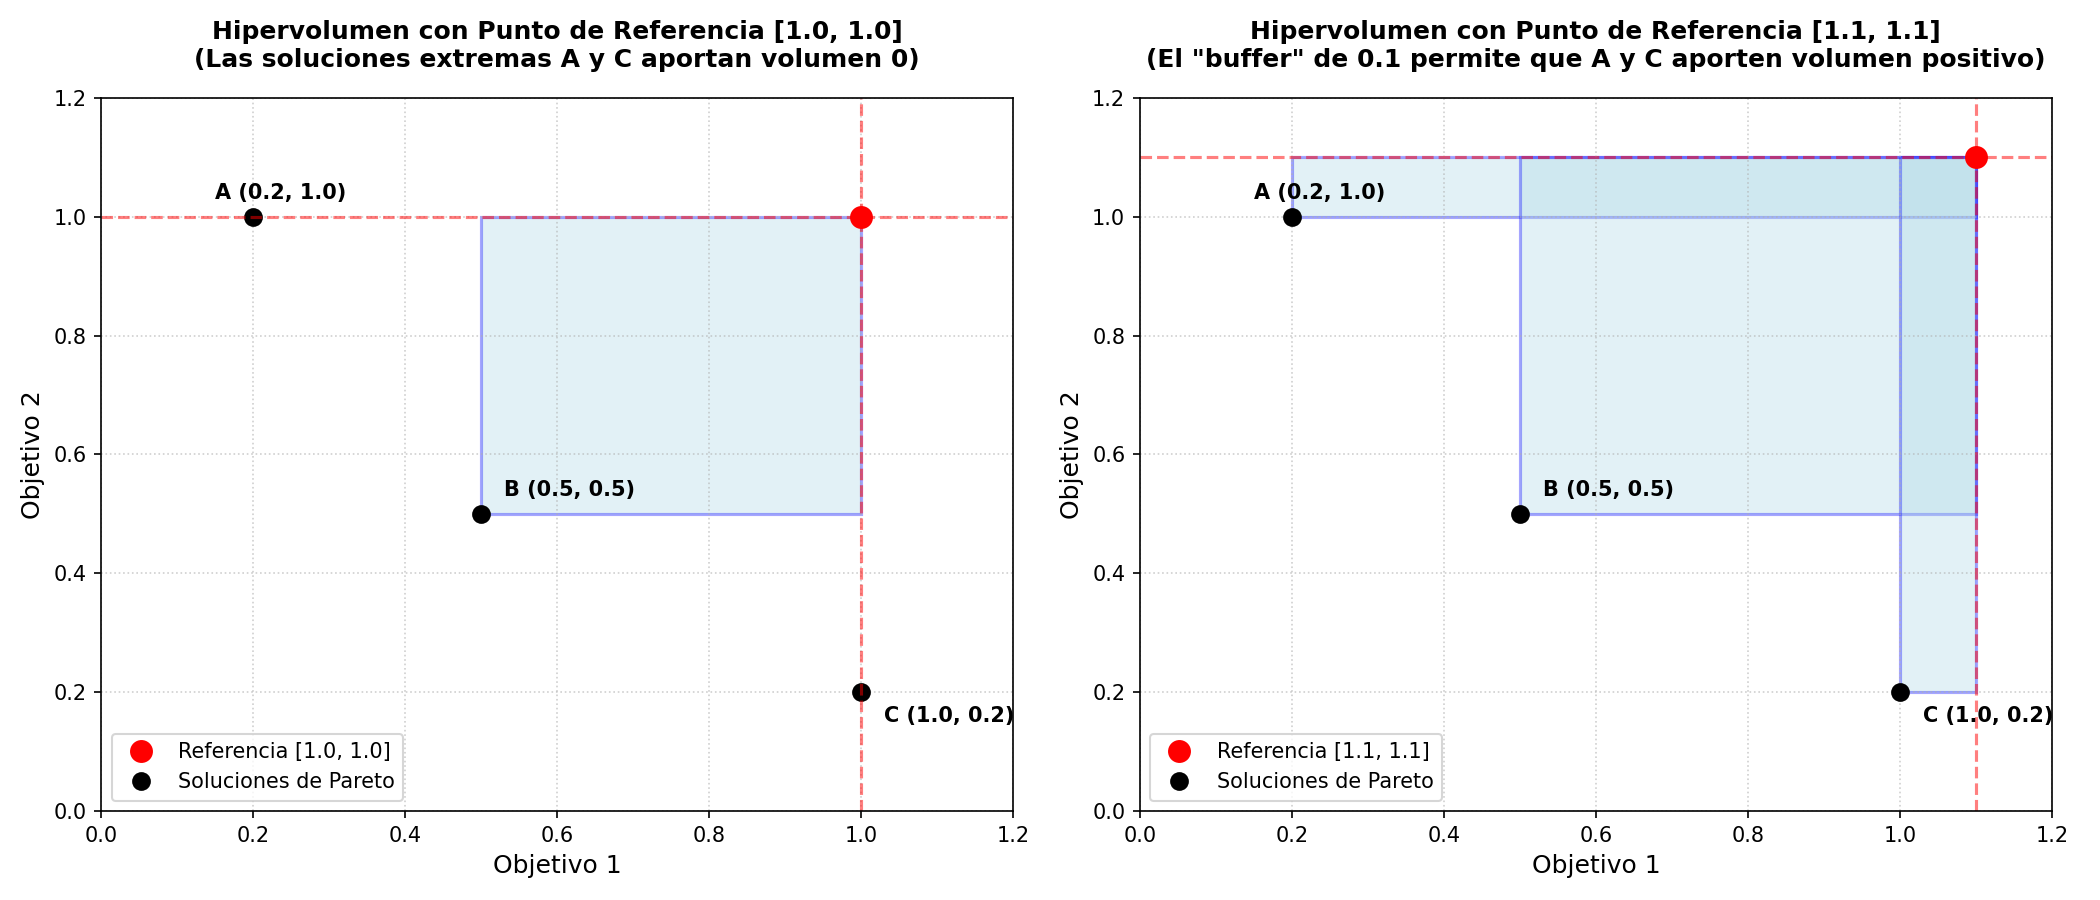
\includegraphics[width=0.9\textwidth]{assets/hv_1.1/hypervolume_comparison_es.png}
    \caption{Comparación geométrica del indicador de hipervolumen con puntos de referencia $[1.0, 1.0]$ (izquierda) y $[1.1, 1.1]$ (derecha). El área sombreada en azul representa el espacio dominado. Se aprecia con claridad cómo el colchón de $0.1$ rescata la aportación de volumen de las soluciones de frontera A y C.}
    \label{fig:hv_comparativa}
\end{figure}

Consideremos una frontera de Pareto compuesta por tres soluciones en un problema de minimización bidimensional:
\begin{itemize}
    \item Solución extrema $A$ en el extremo izquierdo: $A = [0.2, 1.0]$ (excelente en el Objetivo 1, pésimo en el Objetivo 2).
    \item Solución de compromiso $B$ en el centro del frente: $B = [0.5, 0.5]$ (equilibrio entre ambos objetivos).
    \item Solución extrema $C$ en el extremo inferior derecho: $C = [1.0, 0.2]$ (pésimo en el Objetivo 1, excelente en el Objetivo 2).
\end{itemize}

\textbf{Caso 1: Cálculo del hipervolumen con punto de referencia $R = [1.0, 1.0]$}

Calculamos la contribución exclusiva de hipervolumen ($\Delta HV$) de cada solución midiendo el área que \textit{solo} domina esa solución de manera independiente (restando la coordenada de la solución adyacente para no solapar áreas):
\begin{itemize}
    \item Área exclusiva aportada por la solución de frontera $A$:
    \begin{equation}
        \Delta HV(A) = (x_B - x_A) \times (R_y - y_A) = (0.5 - 0.2) \times (1.0 - 1.0) = 0.3 \times 0.0 = 0.0
    \end{equation}
    
    \item Área exclusiva aportada por la solución de frontera $C$:
    \begin{equation}
        \Delta HV(C) = (R_x - x_C) \times (y_B - y_C) = (1.0 - 1.0) \times (0.5 - 0.2) = 0.0 \times 0.3 = 0.0
    \end{equation}
    
    \item Área exclusiva aportada por la solución central $B$:
    \begin{equation}
        \Delta HV(B) = (x_C - x_B) \times (y_A - y_B) = (1.0 - 0.5) \times (1.0 - 0.5) = 0.5 \times 0.5 = 0.25
    \end{equation}
\end{itemize}

\textbf{Resultado:} Las soluciones de frontera $A$ y $C$ quedan completamente borradas del cálculo de volumen debido a que su contribución exclusiva es nula (el producto por cero en su peor dimensión).

\textbf{Caso 2: Cálculo del hipervolumen con punto de referencia $R = [1.1, 1.1]$}

Calculamos nuevamente la contribución exclusiva real ($\Delta HV$) de cada solución con el colchón de $0.1$:
\begin{itemize}
    \item Área exclusiva aportada por la solución de frontera $A$:
    \begin{equation}
        \Delta HV_{buffer}(A) = (x_B - x_A) \times (R_y - y_A) = (0.5 - 0.2) \times (1.1 - 1.0) = 0.3 \times 0.1 = 0.03
    \end{equation}
    
    \item Área exclusiva aportada por la solución de frontera $C$:
    \begin{equation}
        \Delta HV_{buffer}(C) = (R_x - x_C) \times (y_B - y_C) = (1.1 - 1.0) \times (0.5 - 0.2) = 0.1 \times 0.3 = 0.03
    \end{equation}
    
    \item Área exclusiva aportada por la solución central $B$:
    \begin{equation}
        \Delta HV_{buffer}(B) = (x_C - x_B) \times (y_A - y_B) = (1.0 - 0.5) \times (1.0 - 0.5) = 0.5 \times 0.5 = 0.25
    \end{equation}
\end{itemize}

\textbf{Resultado:} Con el punto de referencia $1.1$, las soluciones extremas son plenamente reconocidas por el indicador, aportando un volumen estrictamente positivo de $0.03$ cada una de forma independiente. Dado que el hipervolumen se emplea como una métrica de evaluación de calidad \textit{a posteriori} para evaluar comparativamente el rendimiento de las distintas configuraciones del experimento general, el uso del \textit{buffer} de $0.1$ resulta indispensable. De este modo, se garantiza una valoración justa y no sesgada de aquellos algoritmos que demuestran una excelente capacidad de exploración hacia los extremos de la frontera de Pareto, evitando que sus frentes sean calificados erróneamente con menor calidad debido a una penalización matemática ficticia.

\subsection{Modo de Evaluación: Absoluto vs. Proporcional}

Una decisión de diseño fundamental en la formulación del problema multiobjetivo es el \textbf{modo de evaluación} empleado para calcular los objetivos de tolerancia ($f_2$), distancia media de Hamming ($f_3$) y varianza de balance ($f_4$). El motor evolutivo implementa dos modos mutuamente excluyentes: \textbf{absoluto} y \textbf{proporcional}. Esta sección analiza rigurosamente las implicaciones teóricas y empíricas de cada modo para determinar cuál resulta más apropiado para el experimento general.

\subsubsection{Definición Matemática}

Sea $k$ el número de SNPs seleccionados por un individuo, $D$ el vector de distancias de Hamming entre todos los pares de haplotipos, $\text{minCov} = \min(D)$ la cobertura mínima, $\bar{D}$ la distancia media y $\text{Var}(D)$ la varianza de las distancias.

\textbf{Modo absoluto.} Los objetivos se calculan directamente sobre los valores crudos:
\begin{align}
    f_2^{\text{abs}} &= -\text{minCov}, &
    f_3^{\text{abs}} &= -\bar{D}, &
    f_4^{\text{abs}} &= \text{Var}(D)
\end{align}

\textbf{Modo proporcional} (inspirado en la formulación de Ting \textit{et al.}). Los objetivos se normalizan dividiendo por $k$:
\begin{align}
    f_2^{\text{prop}} &= -\frac{\text{minCov}}{k}, &
    f_3^{\text{prop}} &= -\frac{\bar{D}}{k}, &
    f_4^{\text{prop}} &= \frac{\text{Var}(D)}{k^2}
\end{align}

En ambos casos, el primer objetivo $f_1 = k$ (compactación) permanece inalterado. La transformación proporcional introduce una dependencia matemática explícita entre el tamaño de la solución y el resto de objetivos, lo cual tiene consecuencias profundas sobre la estructura del frente de Pareto resultante.

\subsubsection{Consecuencias Conceptuales}

\textbf{Compresión del espacio fenotípico.} La división por $k$ actúa como un ecualizador que aplana las diferencias absolutas entre soluciones de distinto tamaño. Consideremos dos soluciones hipotéticas:
\begin{itemize}
    \item Solución compacta $A$: $k = 100$, $\text{minCov} = 25$ $\Rightarrow$ $f_2^{\text{prop}} = -0.250$
    \item Solución amplia $B$: $k = 500$, $\text{minCov} = 116$ $\Rightarrow$ $f_2^{\text{prop}} = -0.232$
\end{itemize}

En modo absoluto, estas dos soluciones presentan una separación de $|116 - 25| = 91$ unidades en el eje de tolerancia, lo que permite al algoritmo distinguirlas con claridad y mantener ambas en el frente de Pareto como representantes de regiones fenotípicas radicalmente distintas. Sin embargo, en modo proporcional, la separación se reduce a apenas $|0.250 - 0.232| = 0.018$, comprimiendo soluciones funcionalmente muy diferentes a valores prácticamente indistinguibles.

\textbf{Pérdida de diversidad en la frontera.} Como consecuencia directa de esta compresión, el frente de Pareto en modo proporcional tiende a colapsar hacia una región estrecha del espacio de objetivos. Los algoritmos evolutivos pierden la capacidad de mantener un abanico amplio de soluciones de compromiso, ya que las diferencias entre configuraciones compactas y extensas se diluyen matemáticamente.

\textbf{Inversión de la jerarquía de inicialización.} En modo absoluto, la inicialización \texttt{random\_dense} genera frentes con rangos extensos gracias a la diversidad genética que inyecta en la población inicial. En modo proporcional, la normalización por $k$ neutraliza esta ventaja exploratoria, favoreciendo artificialmente a la inicialización \texttt{greedy\_multi}, cuyas soluciones compactas y homogéneas obtienen proporciones artificialmente elevadas.

\subsubsection{Evidencia Empírica}

Para cuantificar el impacto real de cada modo, se ejecutó un experimento controlado con las mismas configuraciones algorítmicas (NSGA-II, NSGA-III, MOEA/D-TCHE), las mismas dos estrategias de inicialización (\texttt{random\_dense}, \texttt{greedy\_multi}), cruce uniforme (UX), transformación negativa y sin tope de tolerancia ($C = \infty$). La única variable manipulada fue el modo de evaluación.

\begin{table}[H]
\centering
\caption{Comparativa de métricas de calidad entre los modos de evaluación absoluto y proporcional. Cada valor representa la media $\pm$ desviación estándar sobre las 30 ejecuciones totales (6 configuraciones $\times$ 5 semillas).}
\label{tab:abs_vs_prop}
\rowcolors{2}{gray!10}{white}
\begin{tabular}{l c c}
\toprule
\textbf{Métrica} & \textbf{Absoluto} & \textbf{Proporcional} \\
\midrule
Hipervolumen ($\uparrow$) & $0.2669 \pm 0.2230$ & $0.0116 \pm 0.0012$ \\
Rango del frente ($\uparrow$) & $0.9118 \pm 0.6869$ & $0.0840 \pm 0.0638$ \\
Dist. Hamming media ($\uparrow$) & $77.85 \pm 61.05$ & $36.85 \pm 31.44$ \\
Tasa tolerancia media & $0.2064 \pm 0.0145$ & $0.1691 \pm 0.0597$ \\
IGD+ ($\downarrow$) & $0.2077 \pm 0.2133$ & $0.3112 \pm 0.3660$ \\
GD+ ($\downarrow$) & $0.4191 \pm 0.3704$ & $0.4991 \pm 0.3388$ \\
\bottomrule
\end{tabular}
\end{table}

Los resultados revelan diferencias drásticas. El hipervolumen se reduce en un factor de $\sim$23$\times$ al pasar al modo proporcional ($0.267 \rightarrow 0.012$), lo que indica un colapso casi total del volumen dominado por los frentes obtenidos. El rango del frente, que mide la extensión geométrica de la frontera de Pareto, cae en un factor de $\sim$11$\times$ ($0.912 \rightarrow 0.084$), confirmando la compresión fenotípica predicha por el análisis teórico.

\begin{table}[H]
\centering
\caption{Desglose del hipervolumen y rango por configuración algorítmica.}
\label{tab:abs_vs_prop_desglose}
\rowcolors{2}{gray!10}{white}
\begin{tabular}{l l c c c c}
\toprule
 & & \multicolumn{2}{c}{\textbf{Hipervolumen ($\uparrow$)}} & \multicolumn{2}{c}{\textbf{Rango ($\uparrow$)}} \\
\cmidrule(lr){3-4} \cmidrule(lr){5-6}
\textbf{Algoritmo} & \textbf{Inicialización} & \textbf{Abs.} & \textbf{Prop.} & \textbf{Abs.} & \textbf{Prop.} \\
\midrule
NSGA-II & \texttt{random\_dense}  & 0.5344 & 0.0112 & 1.9220 & 0.2084 \\
NSGA-II & \texttt{greedy\_multi}  & 0.0610 & 0.0125 & 0.3338 & 0.0554 \\
NSGA-III & \texttt{random\_dense} & 0.4781 & 0.0115 & 1.3489 & 0.1153 \\
NSGA-III & \texttt{greedy\_multi} & 0.0469 & 0.0125 & 0.2461 & 0.0346 \\
MOEA/D  & \texttt{random\_dense}  & 0.4404 & 0.0091 & 1.4076 & 0.0597 \\
MOEA/D  & \texttt{greedy\_multi}  & 0.0405 & 0.0125 & 0.2121 & 0.0304 \\
\bottomrule
\end{tabular}
\end{table}

Un fenómeno particularmente revelador se observa en la Tabla~\ref{tab:abs_vs_prop_desglose}: en modo proporcional, \textbf{todas las configuraciones convergen a un hipervolumen prácticamente idéntico} ($\approx 0.012$), independientemente del algoritmo o la estrategia de inicialización empleada. Esto sugiere que la normalización por $k$ aplana el paisaje de objetivos hasta el punto de eliminar las diferencias entre configuraciones, anulando la capacidad discriminativa del experimento general.

\subsubsection{Visualización de los Frentes de Pareto}

\begin{figure}[H]
    \centering
    \begin{subfigure}[b]{0.72\textwidth}
        \centering
        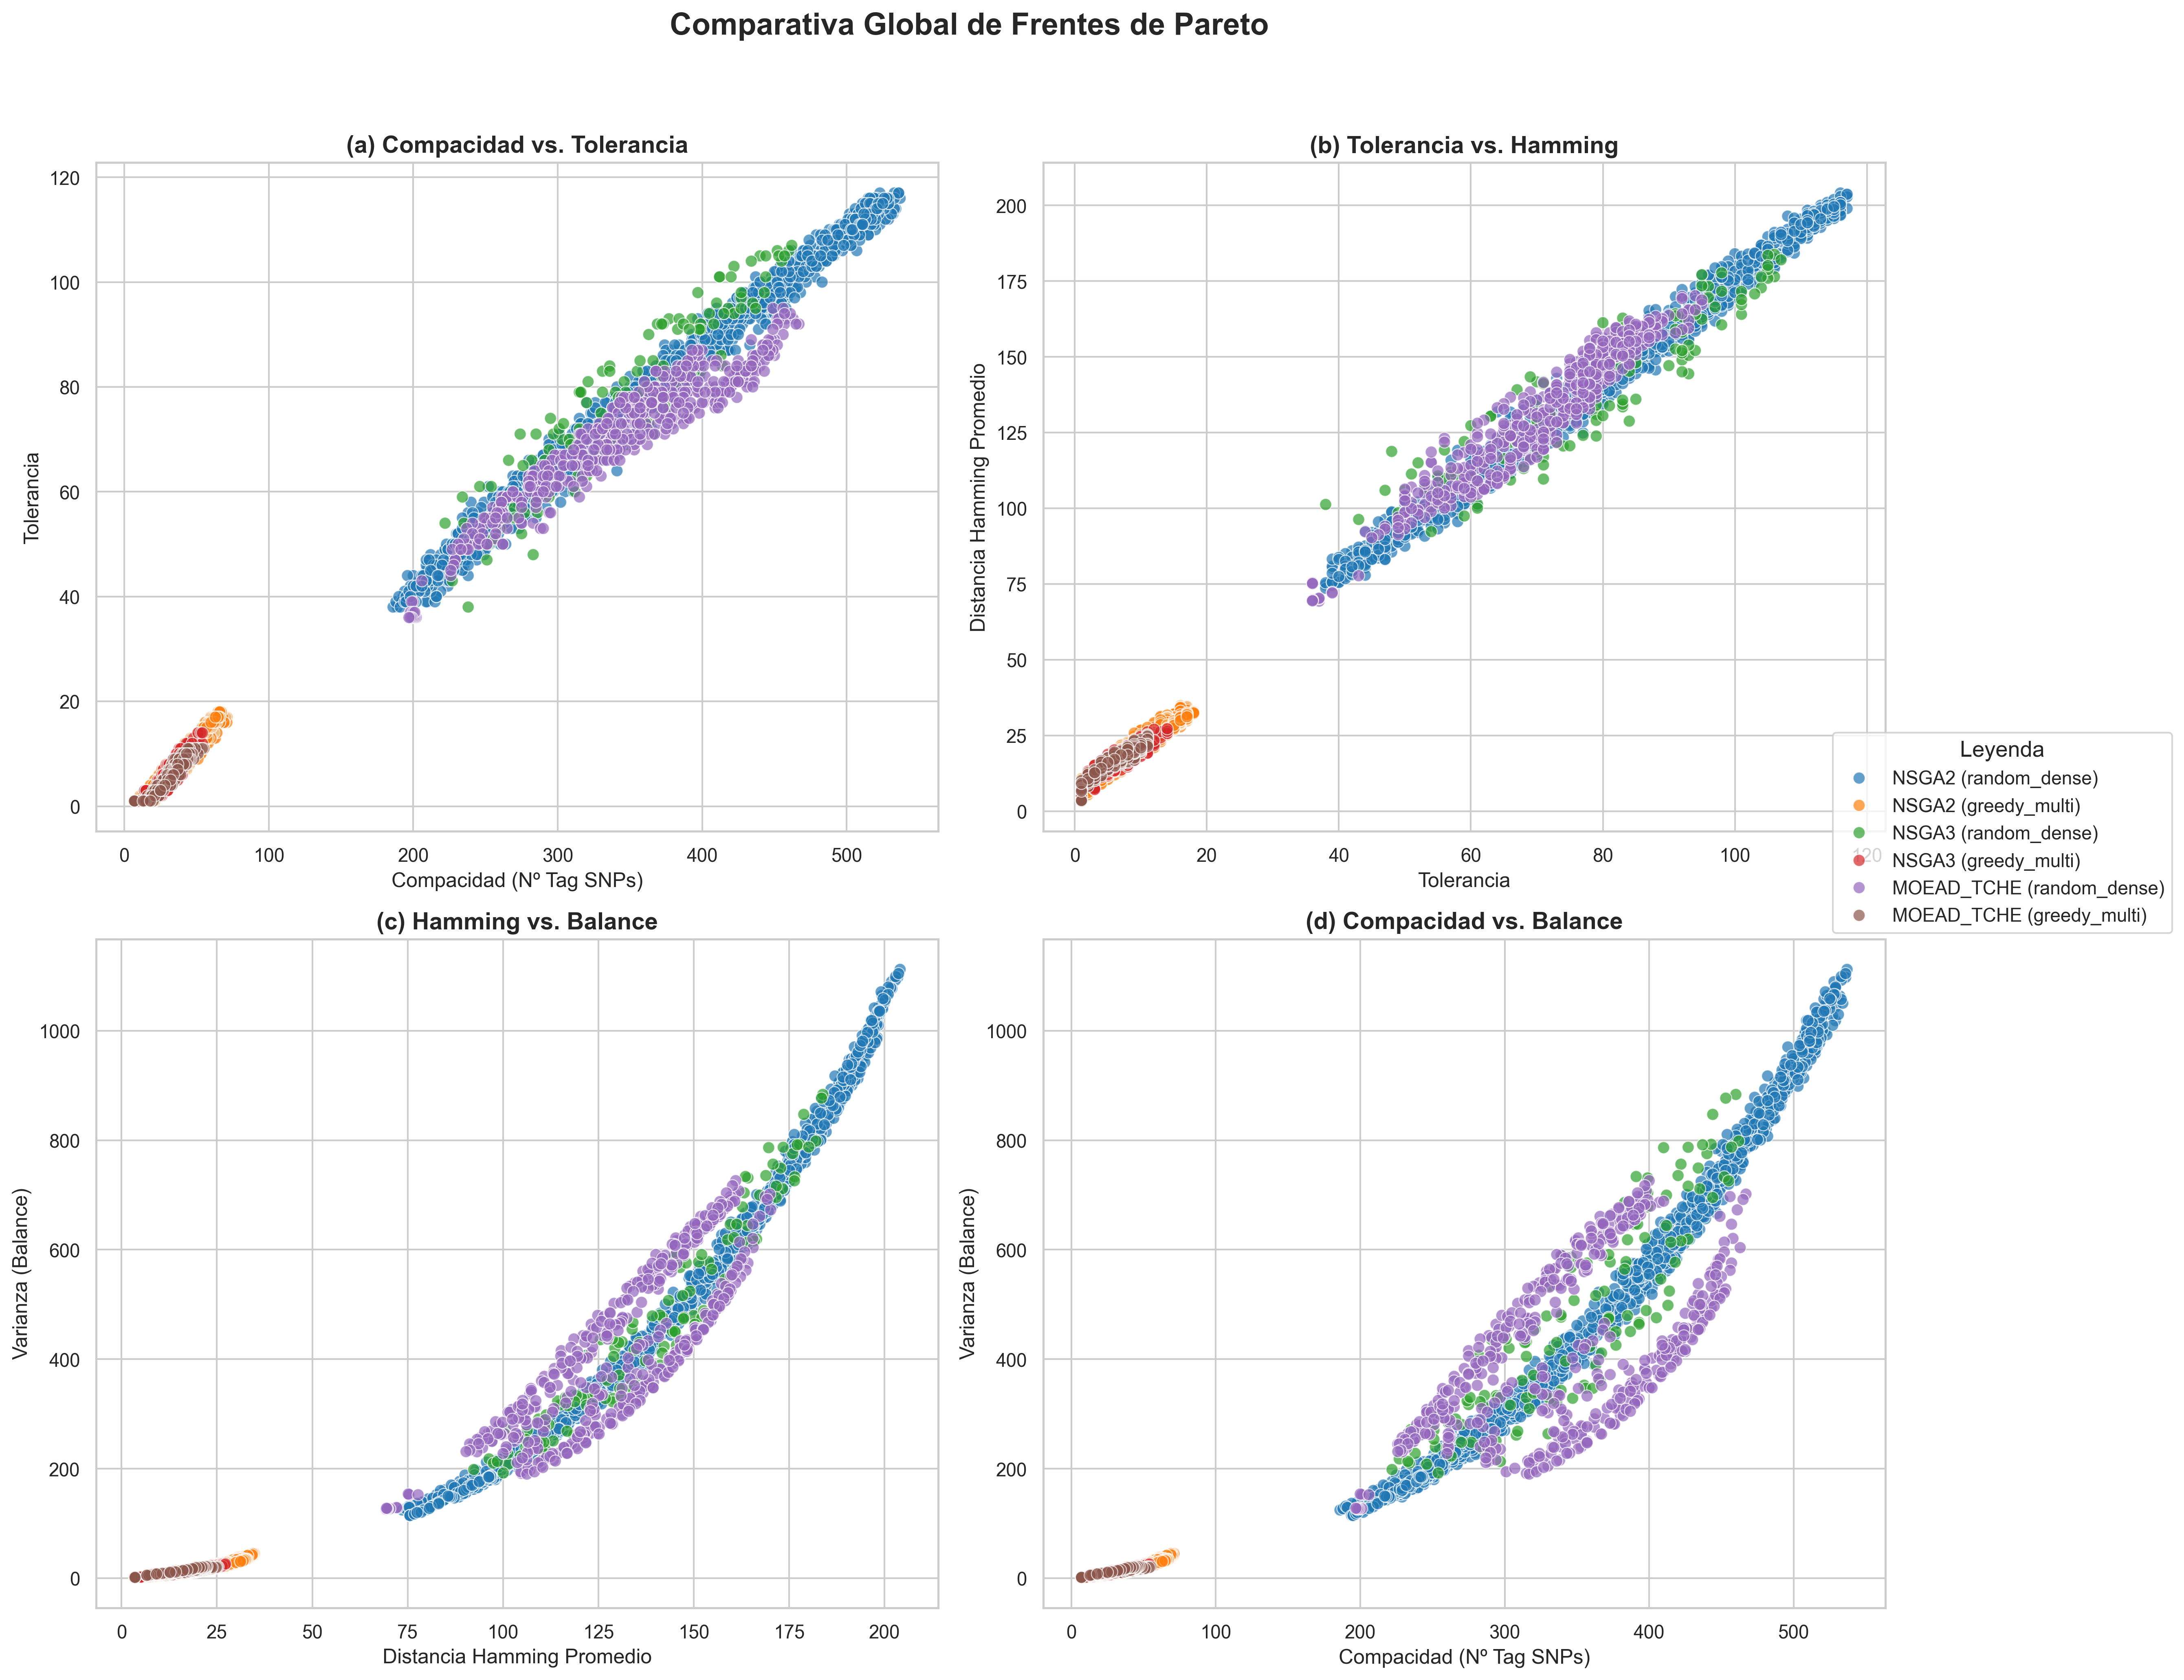
\includegraphics[width=\textwidth]{assets/ev_mode/frentes_pareto_global_abs.png}
        \caption{Modo absoluto.}
        \label{fig:frente_abs}
    \end{subfigure}
    
    \vspace{0.2cm}
    
    \begin{subfigure}[b]{0.72\textwidth}
        \centering
        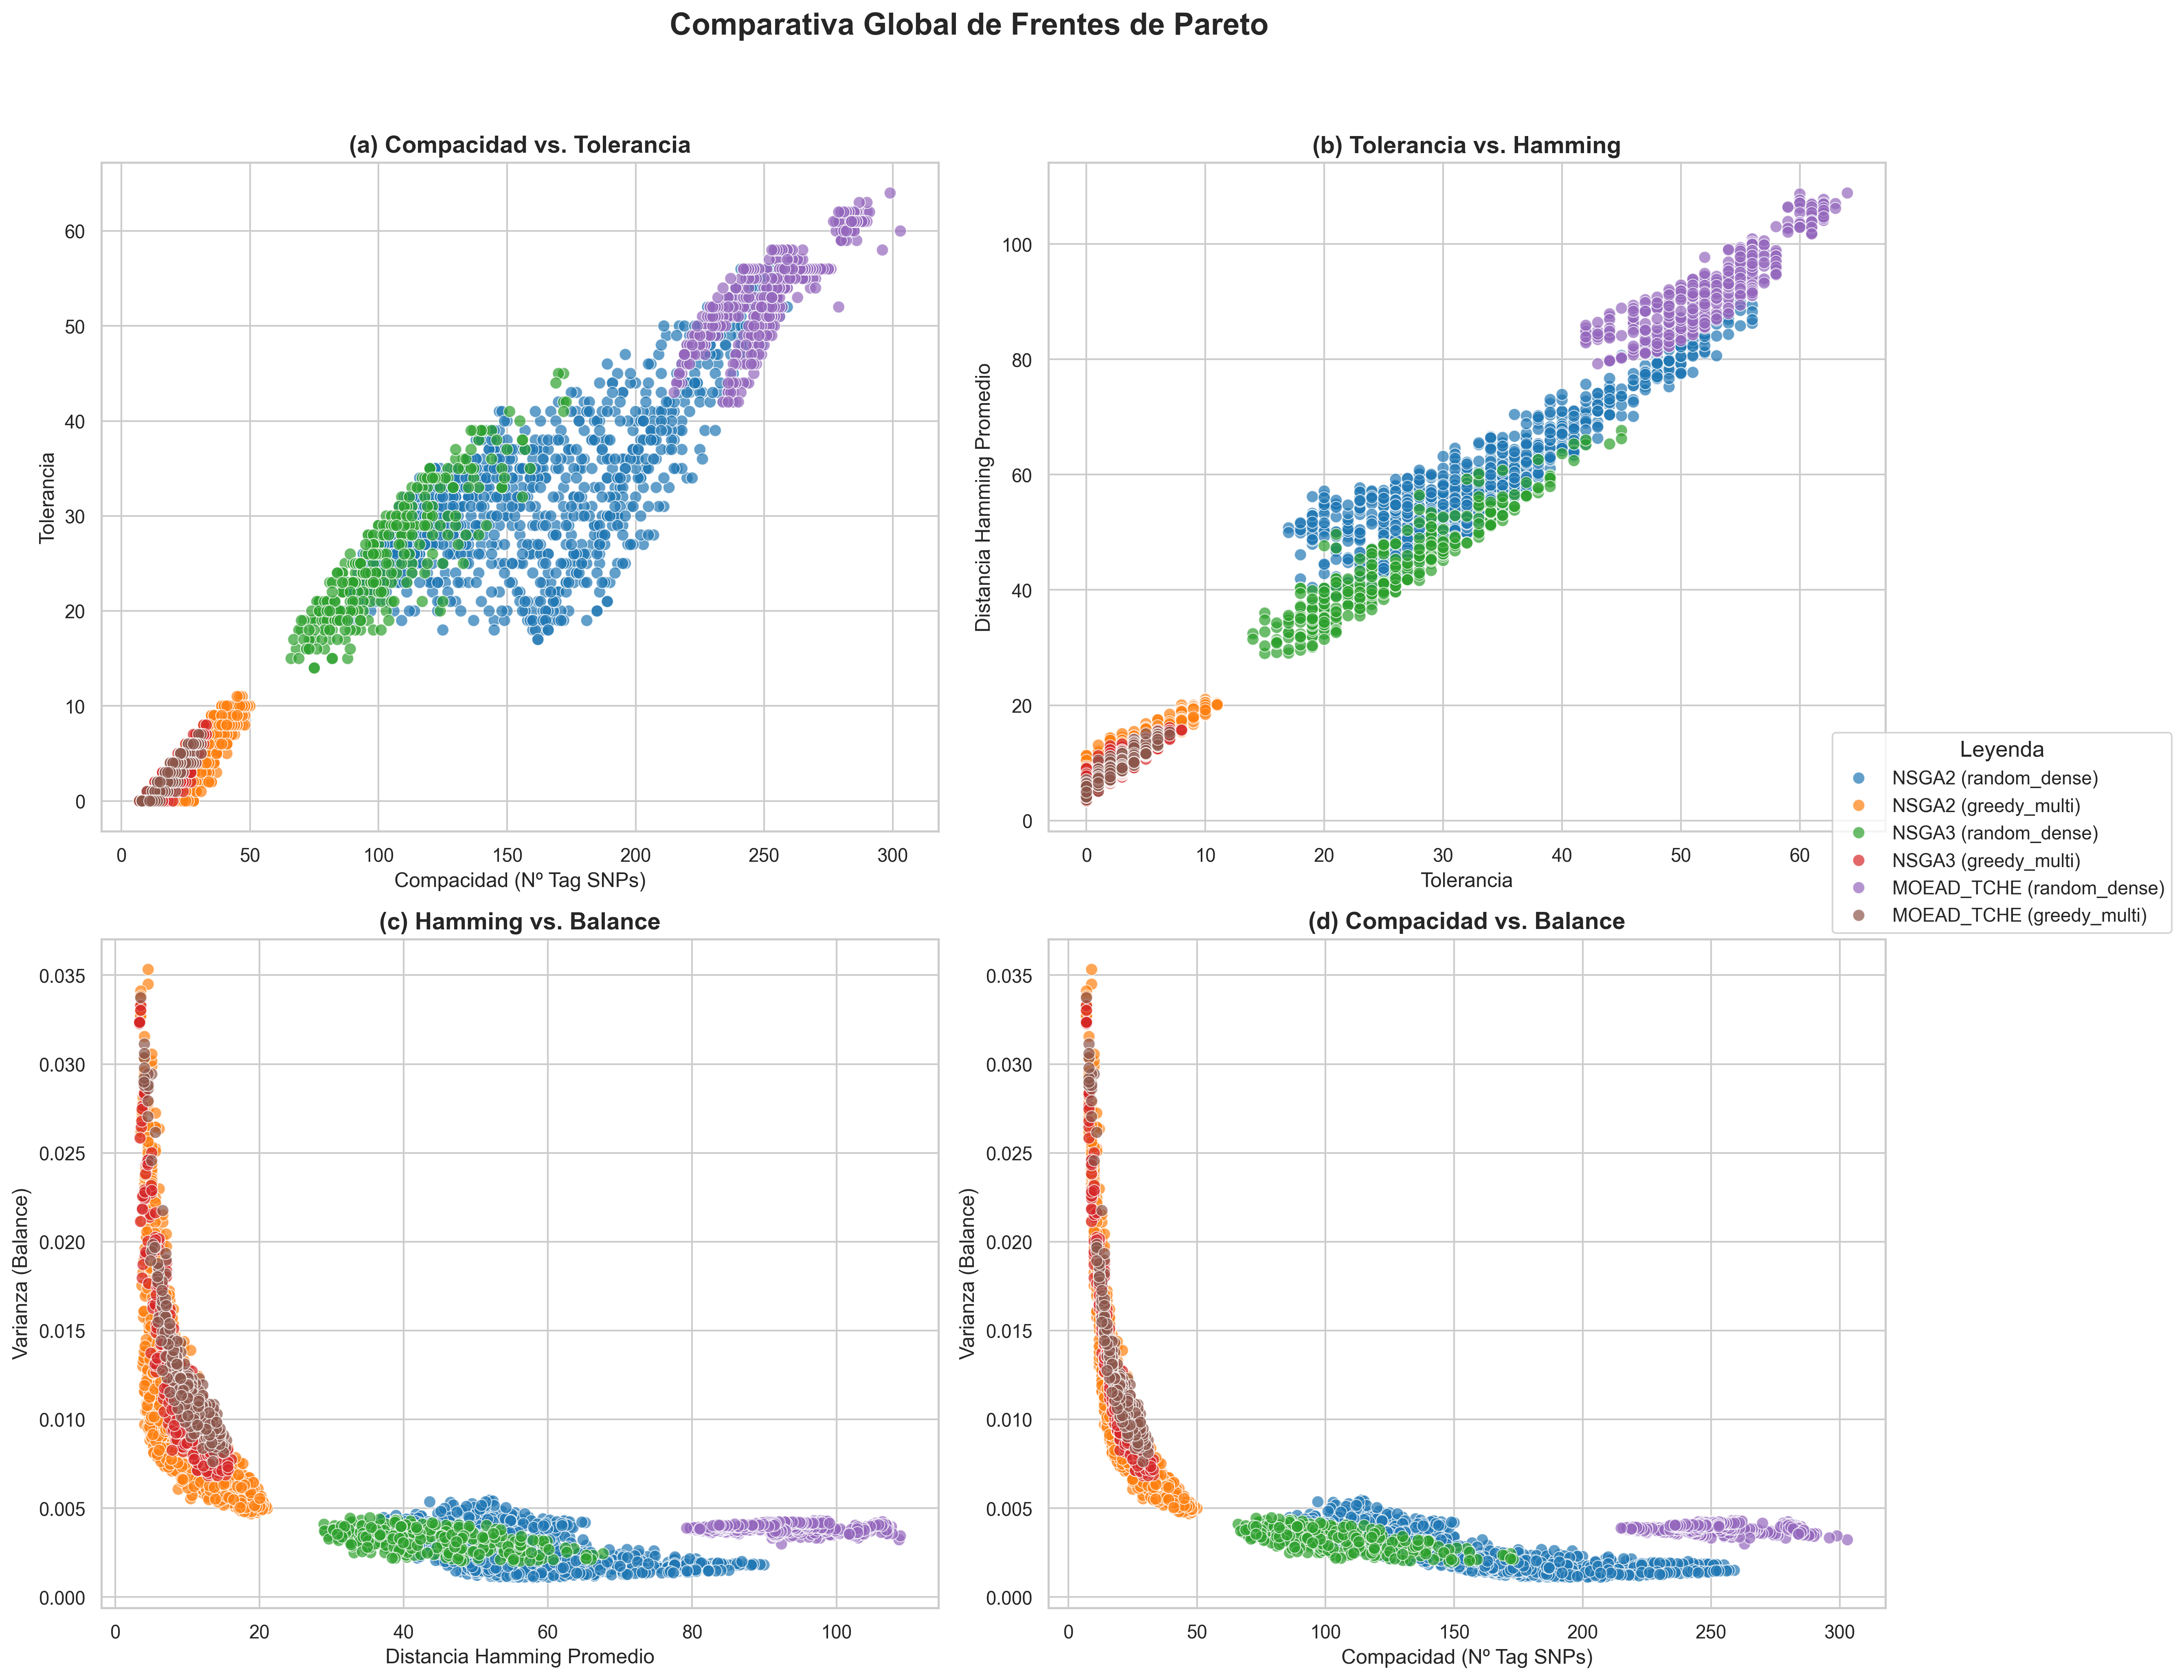
\includegraphics[width=\textwidth]{assets/ev_mode/frentes_pareto_global_prop.png}
        \caption{Modo proporcional.}
        \label{fig:frente_prop}
    \end{subfigure}
    \caption{Comparación de los frentes de Pareto globales obtenidos bajo ambos modos de evaluación (absoluto vs. proporcional). Nótese la diferencia de escala en los ejes y la drástica reducción del rango en el modo proporcional.}
    \label{fig:frentes_abs_vs_prop}
\end{figure}

\paragraph{Análisis General}~\\
El análisis detallado de las gráficas presentadas en la Figura~\ref{fig:frentes_abs_vs_prop} revela fenómenos geométricos importantes derivados de la elección del modo de evaluación. En el modo \textbf{absoluto}, los frentes presentan un rango amplio (valor medio de $0.91 \pm 0.69$) con soluciones distribuidas de forma coherente desde configuraciones compactas (bajo $k$, baja tolerancia) hasta configuraciones extensas (alto $k$, alcanzando valores de más de $500$ SNPs; y alta tolerancia, con valores que se acercan a $120$ SNPs). La evolución sigue una trayectoria monotónica donde tanto la distancia de Hamming como la varianza cruda crecen naturalmente conforme aumenta el tamaño de la solución.

Por el contrario, en el modo \textbf{proporcional}, los frentes colapsan en una banda estrecha (reducción del rango medio a $0.08 \pm 0.06$, lo que supone una drástica caída de $\sim 11\times$), perdiendo diversidad fenotípica y limitando la capacidad de ofrecer un abanico amplio de soluciones de compromiso al decisor. Se alcanzan valores máximos de compacidad inferiores a $300$ SNPs (prácticamente la mitad que en modo absoluto) y valores de tolerancia inferiores a $60$ (también aproximadamente la mitad respecto al modo absoluto).

\paragraph{Análisis de Dispersión del Balance}~\\
Resulta de particular interés el comportamiento de la inicialización \texttt{greedy\_multi} en los gráficos de dispersión (subplots c y d de la figura). En el modo proporcional, los puntos generados por esta heurística se muestran notablemente dispersos a lo largo del eje de la varianza (balance), trazando una curva hiperbólica descendente. Este comportamiento, en contraposición con la compactación observada en el modo absoluto, no constituye un defecto o error de ejecución, sino que representa una consecuencia matemática directa de la normalización aplicada al objetivo de varianza ($f_4 = \frac{\text{Var}(D)}{k^2}$).

La inicialización \texttt{greedy\_multi} explora de forma dirigida un subespacio de soluciones muy compactas ($k \in [7, 50]$), mientras que el enfoque puramente estocástico \texttt{random\_dense} opera inherentemente con soluciones mucho más extensas ($k \in [66, 303]$). Al dividir la varianza absoluta $\text{Var}(D)$ por el cuadrado del tamaño de la solución ($k^2$), la función divisora exhibe una curvatura fuertemente convexa para valores pequeños de $k$. Como se aprecia en la Tabla~\ref{tab:dispersion_greedy}, el divisor experimenta un incremento masivo de $51\times$ al pasar de un $k=7$ (divisor $49$) a un $k=50$ (divisor $2500$). 

\begin{table}[H]
\centering
\caption{Impacto empírico del divisor $k^2$ en la dispersión geométrica del balance para la heurística \texttt{greedy\_multi} (Modo Proporcional).}
\label{tab:dispersion_greedy}
\rowcolors{2}{gray!10}{white}
\resizebox{\textwidth}{!}{%
\begin{tabular}{c c c c}
\toprule
\textbf{Tamaño ($k$)} & \textbf{Divisor ($k^2$)} & \textbf{Rango Balance Proporcional ($f_4$)} & \textbf{Comportamiento visual de los puntos} \\
\midrule
$7$ & $49$ & $[0.0322, 0.0341]$ & Dispersión máxima (banda superior alta) \\
$15$ & $225$ & $[0.0094, 0.0172]$ & Transición de la curva hiperbólica descendente \\
$30$ & $900$ & $[0.0062, 0.0091]$ & Compresión incipiente hacia la banda principal \\
$50$ & $2500$ & $\approx 0.0050$ & Colapso cuasi-puntual por dominancia del divisor \\
\bottomrule
\end{tabular}%
}
\end{table}

Este ``rango'' representa el intervalo $[f_{4,\min}, f_{4,\max}]$ en el que oscilan los valores del objetivo de balance para las soluciones de la frontera de Pareto que poseen exactamente un tamaño de solución $k$ determinado:
\begin{itemize}
    \item \textbf{Para $k = 7$:} El rango es $[0.0322, 0.0341]$. Dado que el divisor es muy reducido ($7^2 = 49$), la varianza proporcional resultante es alta y los puntos se sitúan en la parte superior del gráfico.
    \item \textbf{Para $k = 30$:} El rango decrece notablemente hasta $[0.0062, 0.0091]$ debido a un divisor mucho mayor ($30^2 = 900$), comprimiendo los valores hacia abajo.
    \item \textbf{Para $k = 50$:} El rango prácticamente colapsa a un único punto en torno a $\approx 0.0050$, ya que el divisor de $2500$ neutraliza casi por completo cualquier variación en la varianza cruda.
\end{itemize}
De este modo, el rango de balance proporcional describe la amplitud y magnitud de los valores de varianza normalizada que alcanzan las soluciones para cada nivel de compacidad ($k$).

Este rápido crecimiento del denominador provoca que la varianza proporcional se amplifique drásticamente para las soluciones de menor tamaño, dispersando visualmente el frente y rompiendo la progresión monotónica. Por el contrario, todas las soluciones originadas por \texttt{random\_dense}, al poseer denominadores $k^2$ de varios órdenes de magnitud superiores, comprimen matemáticamente sus varianzas en una densa banda horizontal plana, aglomerando visualmente los puntos.

\subsubsection{Análisis de Ventajas y Desventajas}

\textbf{Ventajas del modo absoluto:}
\begin{itemize}
    \item Preserva la diversidad fenotípica natural del frente de Pareto, ofreciendo al decisor un abanico completo de soluciones de compromiso.
    \item Permite al algoritmo evolutivo discriminar eficazmente entre soluciones de distinto tamaño y calidad, maximizando la utilidad de la búsqueda.
    \item Las configuraciones con inicialización estocástica (\texttt{random\_dense}) pueden explorar regiones extremas del espacio de objetivos, descubriendo soluciones que la inicialización heurística no alcanza.
\end{itemize}

\textbf{Desventajas del modo absoluto:}
\begin{itemize}
    \item Los valores crudos de las métricas pueden sesgar la búsqueda hacia soluciones de mayor tamaño ($k$ alto), ya que las tolerancias absolutas crecen naturalmente con el número de SNPs seleccionados.
\end{itemize}

\textbf{Ventajas del modo proporcional:}
\begin{itemize}
    \item Normaliza los objetivos por el tamaño de la solución, evaluando la \textit{eficiencia por SNP} en lugar de la contribución bruta. Esta formulación tiene fundamento teórico en la literatura (Ting \textit{et al.}).
    \item Facilita la comparación entre soluciones de tamaño muy dispar en términos de su rendimiento relativo.
\end{itemize}

\textbf{Desventajas del modo proporcional:}
\begin{itemize}
    \item Compresión severa del frente de Pareto: el rango se reduce en un factor $\sim$11$\times$ y el hipervolumen en $\sim$23$\times$. Esto supone una desventaja porque diluye matemáticamente las diferencias entre soluciones fenotípicamente distintas (una solución compacta y una extensa pueden colapsar en el mismo valor proporcional), lo que impide al algoritmo conservar y ofrecer un abanico diverso de opciones.
    \item Reduce drásticamente la varianza y las distancias en rendimiento entre configuraciones algorítmicas. La compresión de los datos diluye las diferencias relativas frente a la varianza estocástica de las semillas. Como consecuencia, los p-valores en las pruebas de hipótesis aumentan en varios órdenes de magnitud. Esto se ha comprobado empíricamente mediante ejecuciones auxiliares con 30 semillas independientes (\texttt{full30\_cx}): en la métrica de hipervolumen, el test de Kruskal-Wallis arroja un $p$-valor de $1.81 \times 10^{-11}$ para el modo absoluto, permitiendo al análisis post hoc (Test de Dunn) distinguir significativamente la práctica totalidad de los pares de configuraciones. Por el contrario, en el modo proporcional el $p$-valor asciende hasta $0.0166$, un empeoramiento de $9$ órdenes de magnitud que dificulta el rechazo de la hipótesis nula y se traduce en un mapa de calor dominado por empates técnicos (Figura~\ref{fig:posthoc_abs_vs_prop}).
\end{itemize}

\begin{figure}[H]
    \centering
    \begin{subfigure}[b]{0.48\textwidth}
        \centering
        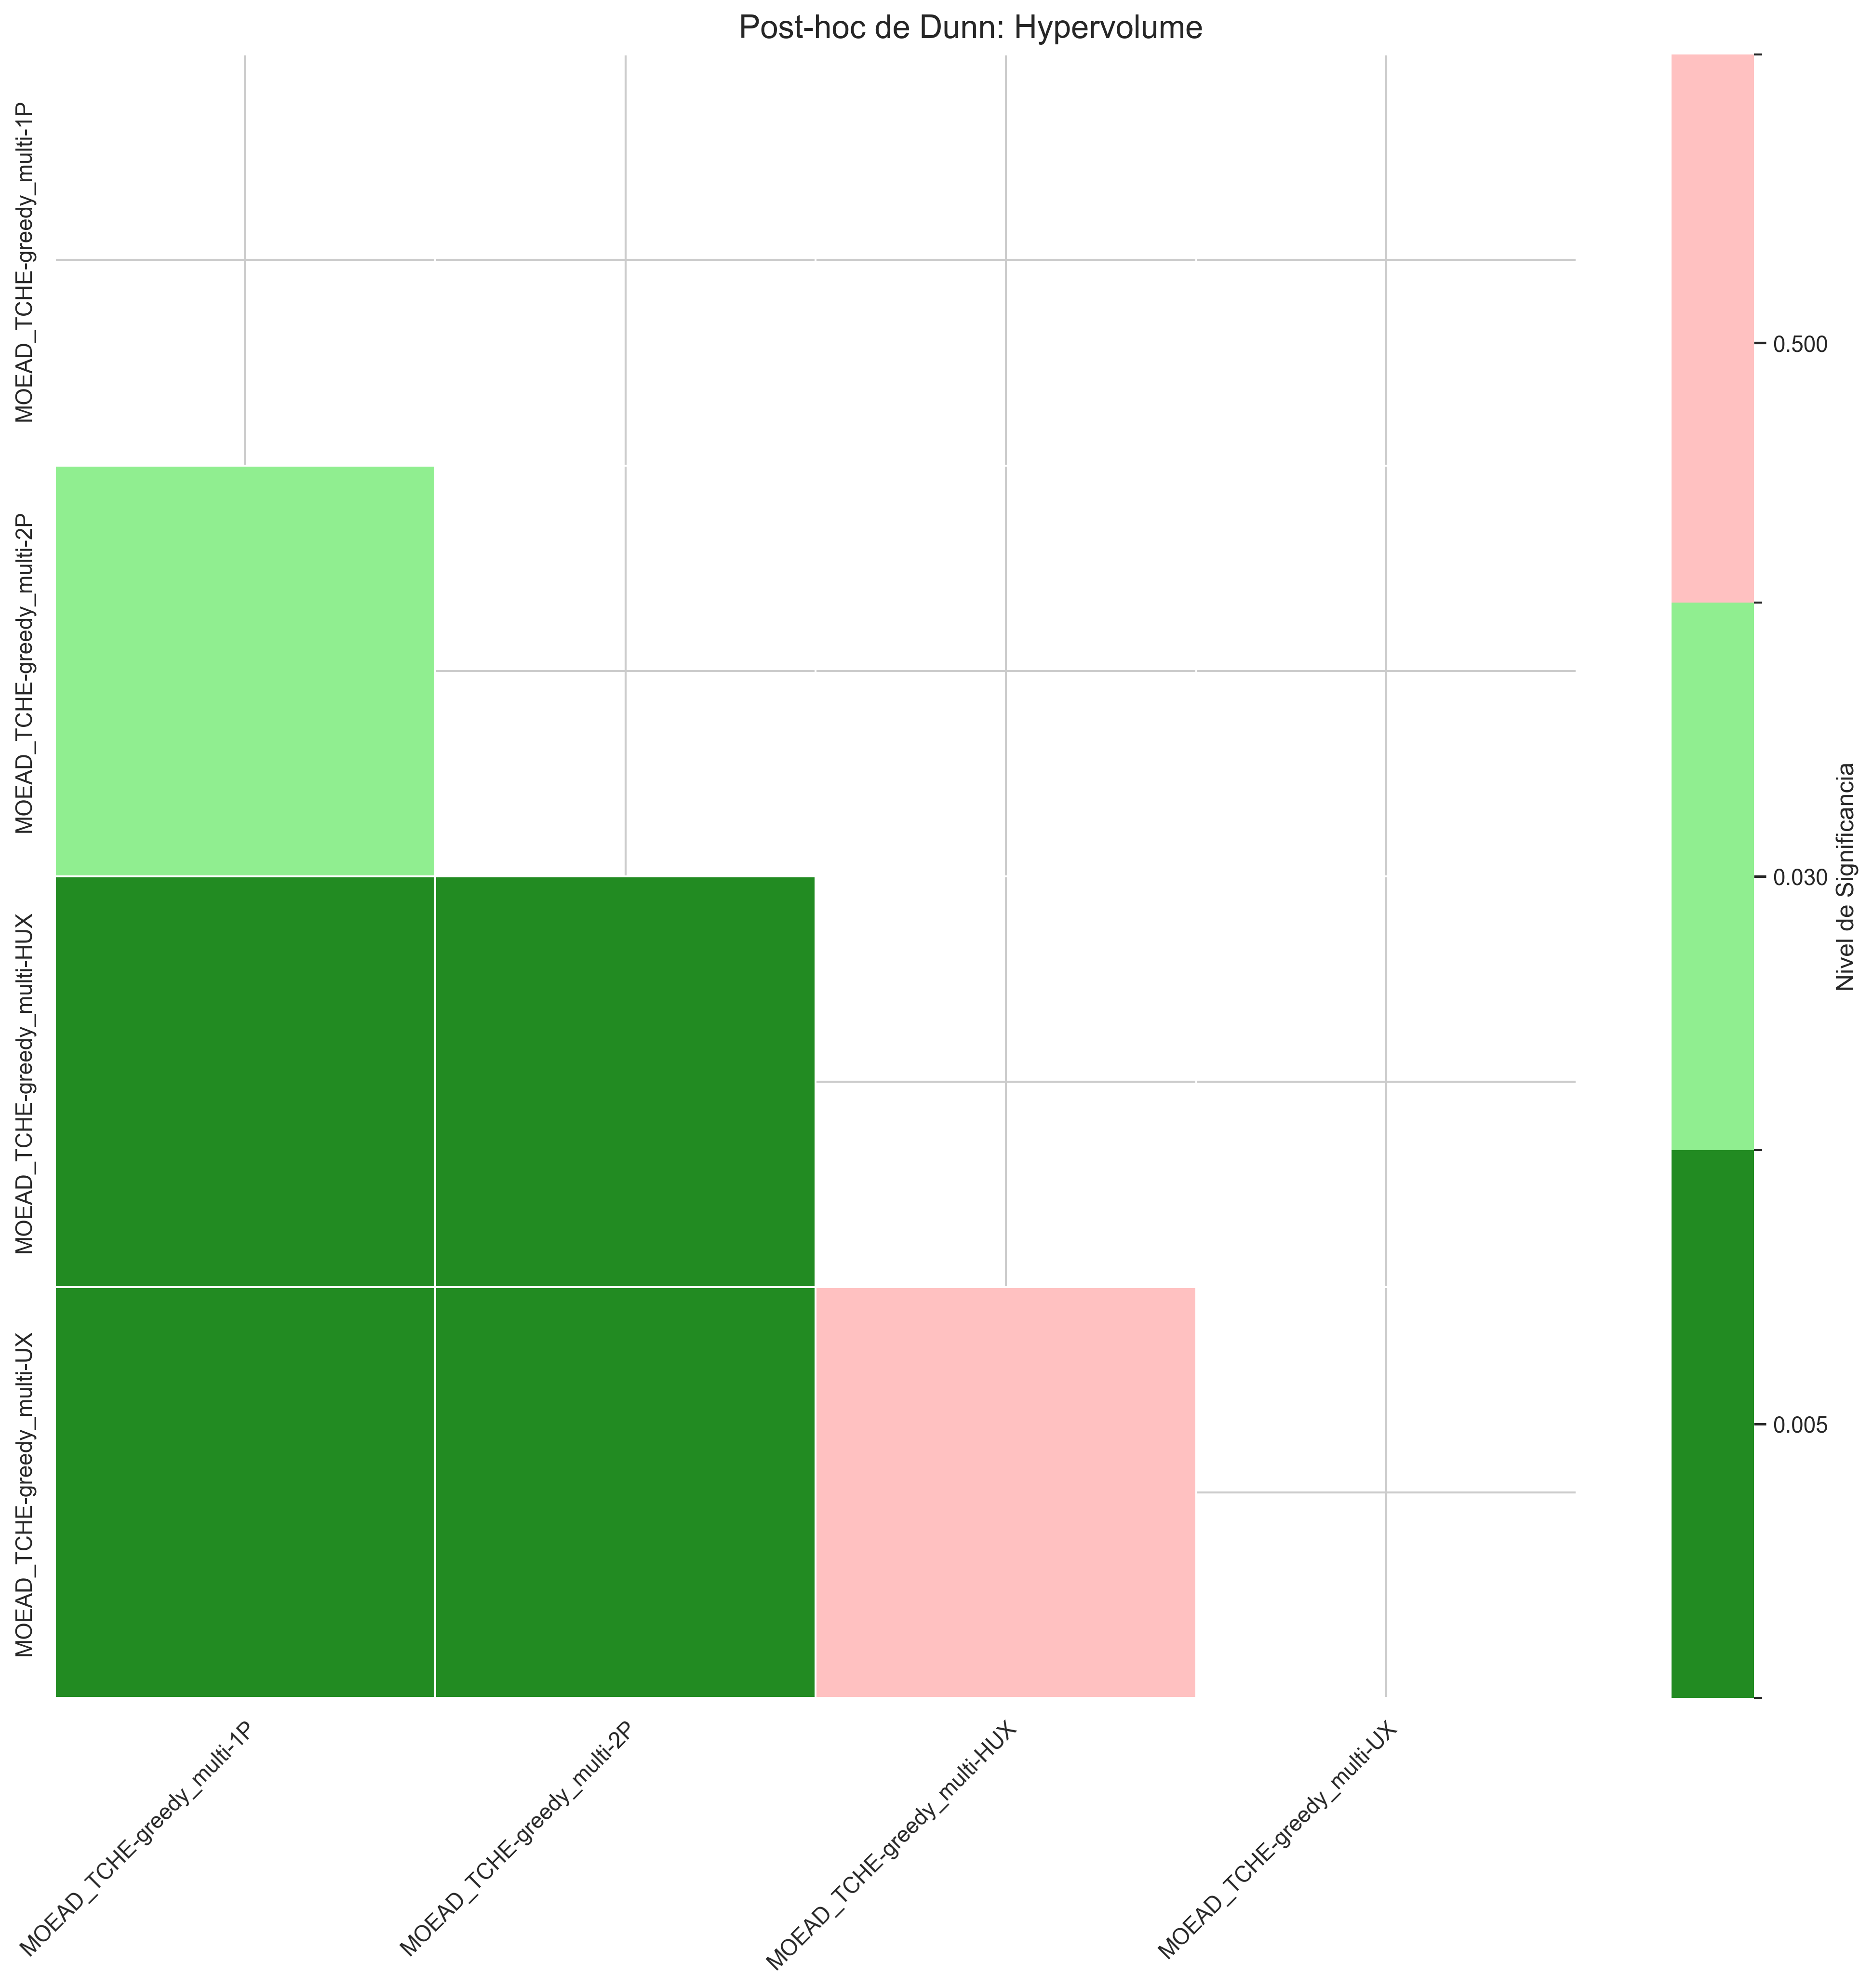
\includegraphics[width=\textwidth]{../exp_auxiliares/full30_cx_negAbs/2_comparativa/4_rankings/estadistica_hv/heatmap_dunn_hypervolume_full_30.png}
        \caption{Test de Dunn (Modo Absoluto)}
        \label{fig:dunn_abs}
    \end{subfigure}
    \hfill
    \begin{subfigure}[b]{0.48\textwidth}
        \centering
        
\includegraphics[width=\textwidth]{../exp_auxiliares/full30_cx_negProp/2_comparativa/4_rankings/estadistica_hv/heatmap_dunn_hypervolume_full_30.png}
        \caption{Test de Dunn (Modo Proporcional)}
        \label{fig:dunn_prop}
    \end{subfigure}
    \caption{Comparativa de la significancia estadística (análisis post hoc mediante el test de Dunn) para la métrica de hipervolumen tras 30 ejecuciones independientes. Las celdas verdes indican diferencias estadísticamente significativas ($p < 0.05$). El modo absoluto (izquierda) identifica múltiples pares significativos (5 de 6 combinaciones), mientras que la compresión del modo proporcional (derecha) eleva los p-valores, asumiendo empate técnico en la gran mayoría de configuraciones (solo 1 par de 6 se considera estadísticamente diferente) debido a la incapacidad de separar matemáticamente las distribuciones frente al ruido estocástico.}
    \label{fig:posthoc_abs_vs_prop}
\end{figure}

\begin{itemize}
    \item Penaliza implícitamente las soluciones extensas, limitando la exploración del espacio de búsqueda.
\end{itemize}

\subsubsection{Observaciones}

\paragraph{Sesgo del Modo Absoluto y Comparativa con Moqa}~\\
La comparativa empírica demuestra que la elección de la formulación matemática define inherentemente qué tipo de soluciones sobreviven en la población, introduciendo sesgos hacia extremos opuestos del espacio de búsqueda. Para evidenciar este fenómeno y comprender por qué Moqa et al. debían estar usando el modo proporcional, se analizan dos métricas clave: \textbf{Avg. Hamming Distance} (diversidad fenotípica) y \textbf{Range} (amplitud del frente).

\subparagraph{1. Análisis de la Distancia de Hamming Media (Avg. Hamming)}~\\
El objetivo Hamming mide la capacidad de la solución para diferenciar patrones haplotípicos distintos.

\begin{itemize}
    \item \textbf{En el estudio de Moqa (Modo Proporcional):} Al estar normalizado por el tamaño de la solución ($k$), mide la ``eficiencia por SNP''. La inicialización experta (\textit{Greedy}), diseñada para maximizar esta eficiencia, compite en igualdad de condiciones e incluso supera a la aleatoria.
    \begin{itemize}
        \item \textbf{1º} SPEA2 (Greedy): $0.94$
        \item \textbf{2º} SPEA2 (Random): $0.91$
    \end{itemize}

    \item \textbf{En la ejecución de prueba (negAbs - Modo Absoluto):} Al no dividir por $k$, el Hamming es un valor bruto. Como \texttt{random\_dense} genera cromosomas sustancialmente más grandes (ej. $\approx 300$ SNPs frente a los $\approx 30$ de \texttt{greedy}), el sumatorio bruto siempre será mayor. El modo absoluto premia la magnitud total de información retenida, permitiendo sobrevivir a soluciones densas independientemente de su redundancia:
    \begin{itemize}
        \item \textbf{1º} SPEA2 (\texttt{random\_dense}): $\approx \mathbf{151.6}$
        \item \dots
        \item \textbf{5º} SPEA2 (\texttt{greedy\_multi}): $\approx \mathbf{21.8}$
    \end{itemize}
\end{itemize}

\subparagraph{2. Análisis del Rango del Frente de Pareto (Range)}~\\
El Range evalúa cómo de extendido y diverso es el conjunto de soluciones (desde las más compactas a las más tolerantes).

\begin{itemize}
    \item \textbf{En el estudio de Moqa (Modo Proporcional):} Las inicializaciones heurísticas logran frentes igual de amplios que las aleatorias.
    \begin{itemize}
        \item \textbf{2º} MOEA/D (Greedy): $2.60$ \textit{(muy cerca del 2.75 de MOEA/D Random)}
        \item \textbf{3º} NSGA-II (Greedy): $2.50$ \textit{(superando al 2.45 de NSGA-II Random)}
    \end{itemize}

    \item \textbf{En la ejecución de prueba (negAbs - Modo Absoluto):} El frente de Pareto se dilata hacia cotas brutas elevadas impulsado por las soluciones gigantescas de la inicialización aleatoria. La heurística \texttt{greedy}, diseñada para ser compacta, no alcanza dichos valores absolutos.
    \begin{itemize}
        \item \textbf{1º} NSGA-II (\texttt{random\_dense}): $\approx \mathbf{1.98}$
        \item \dots
        \item \textbf{5º} NSGA-II (\texttt{greedy\_multi}): $\approx \mathbf{0.33}$
    \end{itemize}
\end{itemize}

\textbf{Conclusión fundamental:} No existe un modo intrínsecamente incorrecto, sino dos lentes matemáticas distintas. El \textbf{modo absoluto} define la aptitud basándose en la \textit{magnitud total} de discriminación, beneficiando a las soluciones redundantes generadas por inicializaciones densas. Por el contrario, el \textbf{modo proporcional} (presumiblemente usado por Moqa) define la aptitud basándose en la \textit{eficiencia marginal por SNP}. Su fuerte penalización matemática por tamaño aplasta el rendimiento relativo de las soluciones extensas y amplifica el de las compactas, alineándose perfectamente con la naturaleza de la heurística \textit{Greedy}. Esto explica de forma rigurosa por qué en su estudio ambas inicializaciones compiten en igualdad de condiciones, mientras que en un entorno absoluto la aleatoria domina por acumulación bruta.

\subsubsection{Conclusión}

La elección del modo de evaluación determina fundamentalmente la naturaleza de los frentes de Pareto obtenidos y, por extensión, la utilidad práctica de los resultados del experimento general. El modo absoluto favorece la generación de un espectro amplio de soluciones de compromiso, maximizando la diversidad y la capacidad exploratoria del algoritmo evolutivo. El modo proporcional, en cambio, ofrece una perspectiva de eficiencia normalizada por SNP, pero a un coste empírico muy elevado en términos de compresión del frente y pérdida de discriminación entre configuraciones.

Se deja la decisión final a tu criterio, presentando ambos enfoques con sus respectivos fundamentos teóricos y evidencias empíricas.

\subsection{Transformación de Objetivos: Negación vs. Inversión}

Además del modo de evaluación (absoluto vs. proporcional), otra decisión de diseño con consecuencias profundas sobre la dinámica evolutiva es la \textbf{función de transformación} empleada para convertir los objetivos de maximización (tolerancia $c$ y distancia de Hamming $h$) en objetivos de minimización compatibles con los MOEAs. El motor evolutivo implementa dos opciones: la \textbf{negación lineal} ($f_2 = -c$, $f_3 = -h$) y la \textbf{inversión recíproca} ($f_2 = \frac{1}{c}$, $f_3 = \frac{1}{h}$). En las ejecuciones realizadas con modo absoluto se ha observado que el cambio de transformación provoca una \textbf{inversión completa del ranking de estrategias de inicialización}: la negación favorece a \texttt{random\_dense}, mientras que la inversión favorece a \texttt{greedy\_multi}. La comprensión exhaustiva de este fenómeno requiere un análisis más profundo del que se aborda en este documento.

\begin{table}[H]
\centering
\caption{Inversión del ranking de inicialización según la transformación aplicada. Se muestra el hipervolumen medio por configuración (modo absoluto, cruce UX).}
\label{tab:neg_vs_inv}
\rowcolors{2}{gray!10}{white}
\begin{tabular}{l l c c}
\toprule
\textbf{Algoritmo} & \textbf{Inicialización} & \textbf{Negación (HV)} & \textbf{Inversión (HV)} \\
\midrule
NSGA-II & \texttt{random\_dense}  & \textbf{0.534} (1º) & 1.135 (4º) \\
NSGA-II & \texttt{greedy\_multi}  & 0.061 (4º) & \textbf{1.323} (1º) \\
NSGA-III & \texttt{random\_dense} & 0.478 (2º) & 1.009 (5º) \\
NSGA-III & \texttt{greedy\_multi} & 0.047 (5º) & 1.206 (3º) \\
MOEA/D  & \texttt{random\_dense}  & 0.440 (3º) & 0.933 (6º) \\
MOEA/D  & \texttt{greedy\_multi}  & 0.041 (6º) & 1.273 (2º) \\
\bottomrule
\end{tabular}
\end{table}

Estuve investigando sobre este suceso que tratamos en la última reunión (14/5/26) pero no logré comprender en profundidad la causa del mismo, así que comento brevemente una posible explicación propuesta por Claude Opus 4.6. Según este modelo de IA, el mecanismo subyacente de esta inversión radica en la \textbf{distorsión no lineal del espacio de objetivos} introducida por la función recíproca $\frac{1}{x}$. A diferencia de la negación, que preserva las distancias relativas entre soluciones de forma uniforme (su derivada $\frac{df}{dc} = -1$ es constante), la inversión genera un paisaje asimétrico: comprime drásticamente la zona de alta cobertura donde operan las soluciones de \texttt{greedy\_multi} (la derivada $\frac{df}{dc} = -c^{-2}$ tiende a cero para valores grandes de $c$), mientras que estira enormemente la zona de baja cobertura donde se sitúan las soluciones de \texttt{random\_dense}. Como consecuencia, el cálculo de la \textit{crowding distance} en algoritmos como NSGA-II se ve alterado: las soluciones greedy, agrupadas en una meseta asintótica comprimida, reciben una protección implícita frente a la eliminación por diversidad, mientras que las soluciones aleatorias, dispersas en la zona de gradiente extremo, quedan sometidas a una presión selectiva desproporcionada que consume presupuesto evolutivo en escapar de regiones de baja calidad.

Cabe señalar que este efecto \textbf{no} se debe a limitaciones de precisión numérica en la representación en coma flotante de los valores recíprocos, como se consideró durante la reunión. La arquitectura estándar IEEE 754 de doble precisión (64 bits) maneja con exactitud absoluta cualquier valor recíproco generado en este problema. Incluso en el caso extremo e hipotético de que una solución seleccionase la totalidad de los $1032$ SNPs del dataset Hinds2005 (alcanzando una cobertura o distancia máxima teórica de $1032$), el valor recíproco más pequeño resultante sería $\frac{1}{1032} \approx 9.69 \times 10^{-4}$. Este valor es perfectamente representable y se encuentra sumamente lejos de los límites de precisión y subdesbordamiento (\textit{underflow}) del formato ($\approx 10^{-308}$). El fenómeno observado es, por lo tanto, de naturaleza puramente matemática y algorítmica, no computacional.


\subsection{Número de runs}

Para determinar el número óptimo de ejecuciones independientes (runs) por configuración, se realizaron dos experimentos auxiliares idénticos en modo absoluto con transformación negación (\texttt{full20\_cx\_negAbs} y \texttt{full30\_cx\_negAbs}), variando únicamente el número de semillas: 20 y 30, respectivamente.

\subsubsection{Estabilidad del ranking}

El ranking global de configuraciones se mantiene idéntico en ambos casos (UX $>$ HUX $>$ 2P $>$ 1P), y las medias y desviaciones típicas del hipervolumen son prácticamente indistinguibles:

\begin{table}[H]
\centering
\begin{tabular}{lcc}
\toprule
\textbf{Configuración} & \textbf{HV (20 runs)} & \textbf{HV (30 runs)} \\
\midrule
UX  & $0.0417 \pm 0.0034$ & $0.0410 \pm 0.0041$ \\
HUX & $0.0402 \pm 0.0041$ & $0.0405 \pm 0.0031$ \\
2P  & $0.0370 \pm 0.0026$ & $0.0373 \pm 0.0030$ \\
1P  & $0.0341 \pm 0.0026$ & $0.0338 \pm 0.0033$ \\
\bottomrule
\end{tabular}
\caption{Hipervolumen medio ($\pm$ desviación típica) por operador de cruce con 20 y 30 runs.}
\label{tab:hv_20vs30}
\end{table}

\subsubsection{Significancia estadística}

\paragraph{Test ómnibus (Kruskal-Wallis).}
Ambos experimentos alcanzan significancia estadística en la métrica de hipervolumen, si bien la potencia mejora con 30 runs:
\begin{itemize}
    \item \textbf{20 runs}: $H = 38.37$, $p = 2.37 \times 10^{-8}$.
    \item \textbf{30 runs}: $H = 53.03$, $p = 1.81 \times 10^{-11}$.
\end{itemize}

\paragraph{Análisis post hoc por pares (Test de Dunn).}
La diferencia más relevante entre ambas configuraciones se manifiesta en la capacidad de discriminación par a par. Con 4 operadores de cruce existen $\binom{4}{2} = 6$ pares posibles. El test de Dunn con corrección de Bonferroni revela:
\begin{itemize}
    \item \textbf{20 runs}: \textbf{3 de 6} pares distinguidos significativamente (50\%).
    \item \textbf{30 runs}: \textbf{5 de 6} pares distinguidos significativamente (83\%). El único par no discriminado es UX vs HUX, cuyos rendimientos son efectivamente equivalentes al tratarse de dos variantes del cruce uniforme.
\end{itemize}

Este salto de 50\% a 83\% en la tasa de discriminación constituye la ganancia más tangible de incrementar el número de runs, ya que permite establecer con rigor estadístico la jerarquía completa entre operadores (Figura~\ref{fig:dunn_20vs30_hv}).

\begin{figure}[H]
    \centering
    \begin{subfigure}[b]{0.48\textwidth}
        \centering
        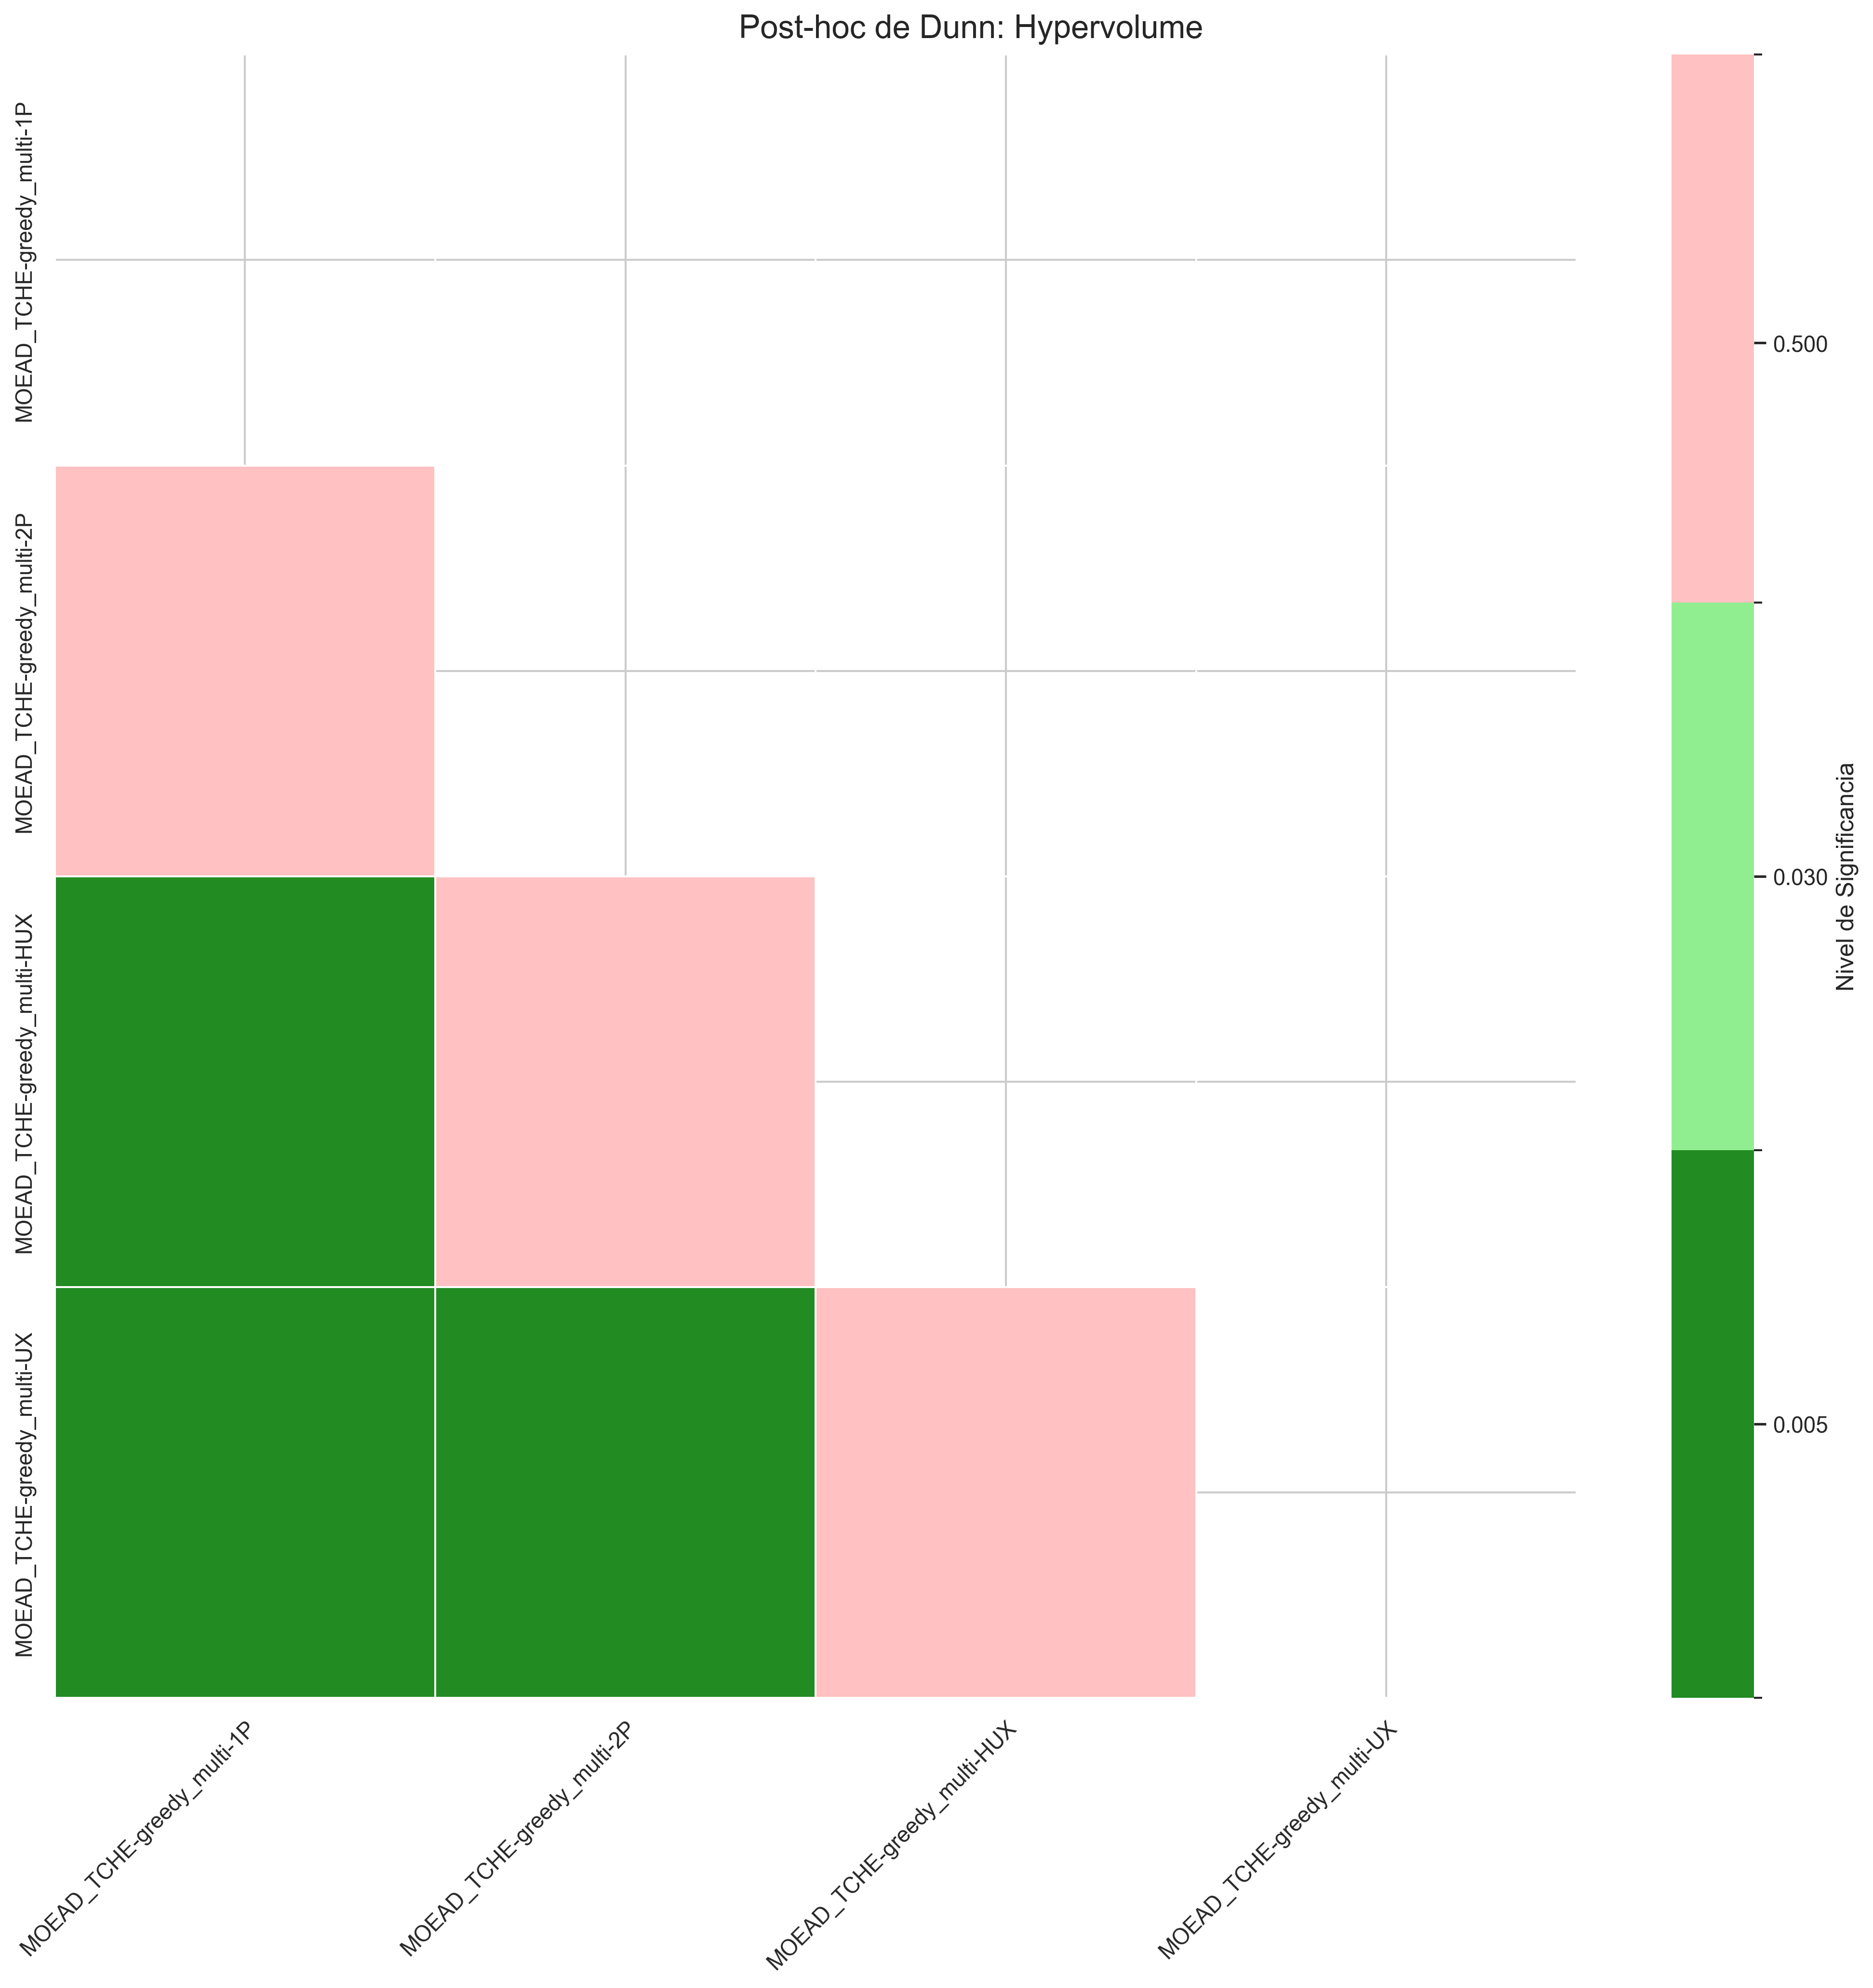
\includegraphics[width=\textwidth]{../exp_auxiliares/full20_cx_negAbs/2_comparativa/4_rankings/estadistica_hv/heatmap_dunn_hypervolume_full_20.png}
        \caption{Test de Dunn con 20 runs}
        \label{fig:dunn_hv_20runs}
    \end{subfigure}
    \hfill
    \begin{subfigure}[b]{0.48\textwidth}
        \centering
        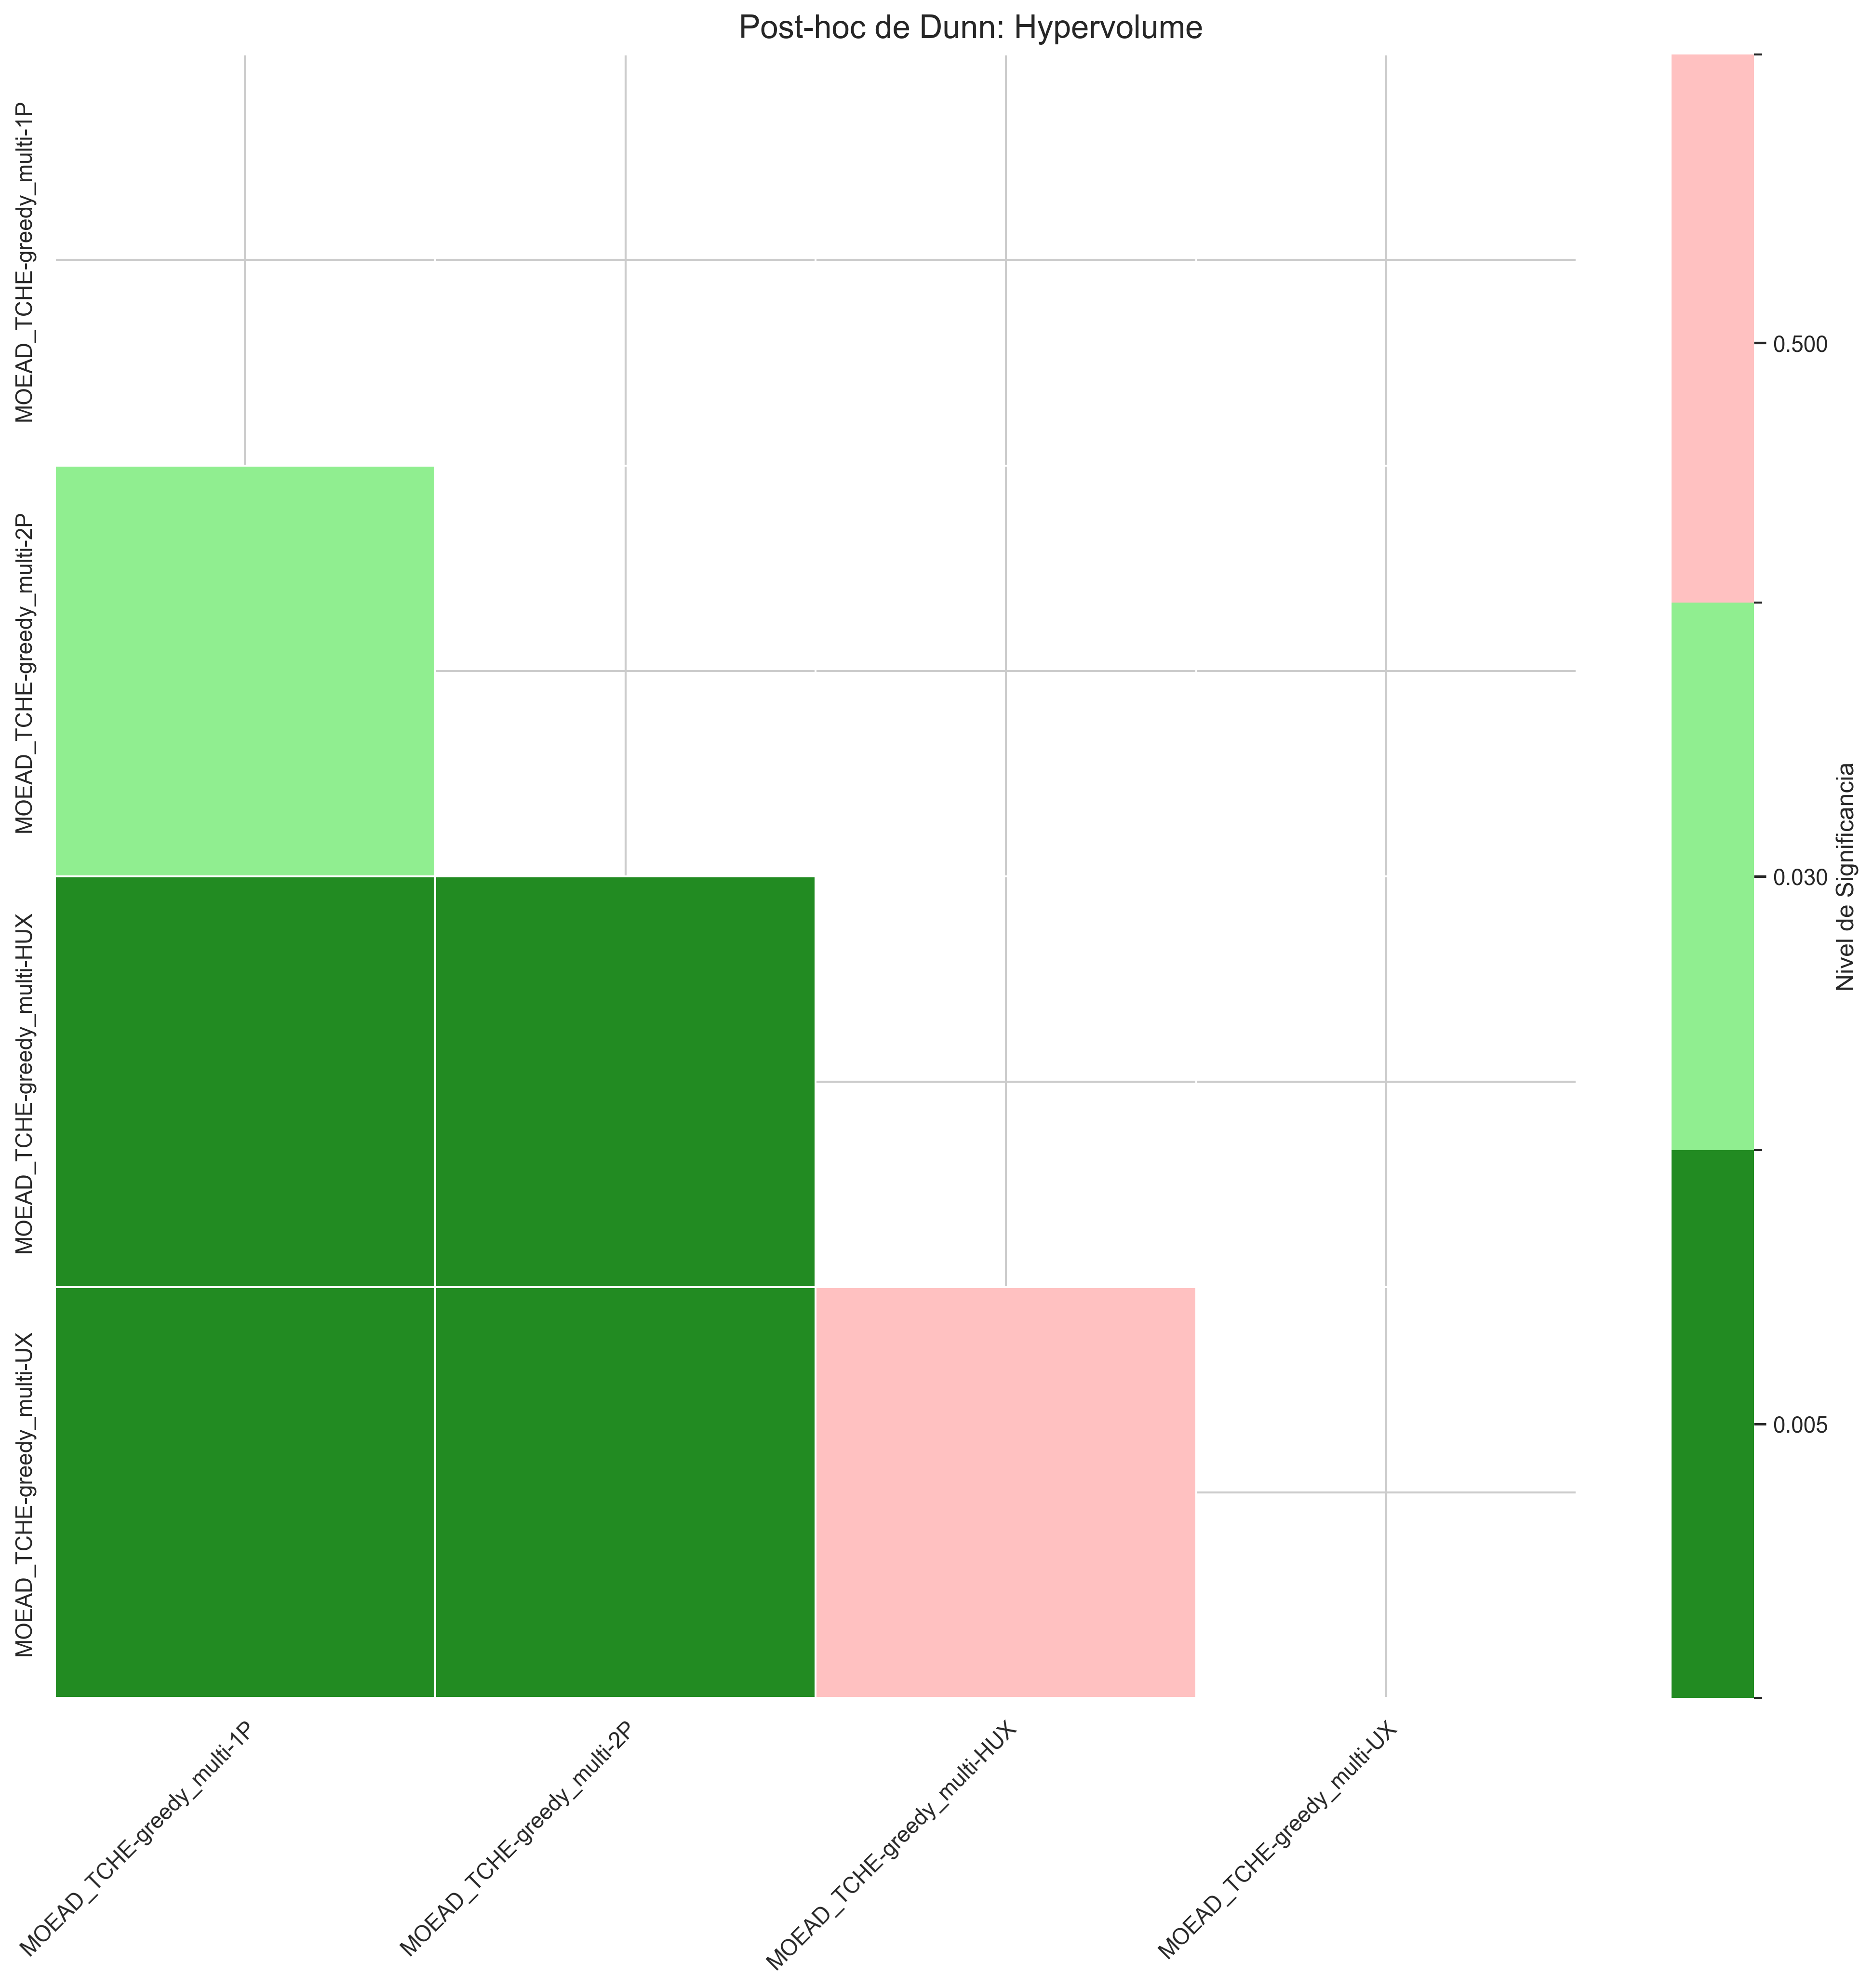
\includegraphics[width=\textwidth]{../exp_auxiliares/full30_cx_negAbs/2_comparativa/4_rankings/estadistica_hv/heatmap_dunn_hypervolume_full_30.png}
        \caption{Test de Dunn con 30 runs}
        \label{fig:dunn_hv_30runs}
    \end{subfigure}
    \caption{Comparativa del análisis post hoc (Test de Dunn) para el hipervolumen con 20 y 30 runs. Las celdas verdes indican pares con diferencias estadísticamente significativas ($p < 0.05$). Con 20 runs se distinguen 3 de 6 pares (50\%), mientras que con 30 runs se alcanzan 5 de 6 (83\%).}
    \label{fig:dunn_20vs30_hv}
\end{figure}

\paragraph{Confirmación con otras métricas (Avg Tolerance Rate).}
Este patrón de mayor capacidad de discriminación al aumentar el tamaño muestral se corrobora empíricamente en otras métricas. Por ejemplo, al analizar el \textit{Average Tolerance Rate}:
\begin{itemize}
    \item \textbf{Test ómnibus (Kruskal-Wallis)}: La significancia estadística general mejora de $p = 4.39 \times 10^{-4}$ ($H = 18.00$) con 20 runs a $p = 2.24 \times 10^{-4}$ ($H = 19.41$) con 30 runs.
    \item \textbf{Test de Dunn}: Con 20 runs únicamente se logran distinguir de forma significativa \textbf{2 de 6} pares (UX vs 1P y HUX vs 1P). Sin embargo, con 30 runs, la reducción de la varianza del error estándar permite descubrir un tercer par (\textbf{3 de 6}), revelando que el operador 2P también es estadísticamente superior a 1P en la tasa media de tolerancia (Figura~\ref{fig:dunn_20vs30_atr}).
\end{itemize}

\begin{figure}[H]
    \centering
    \begin{subfigure}[b]{0.48\textwidth}
        \centering
        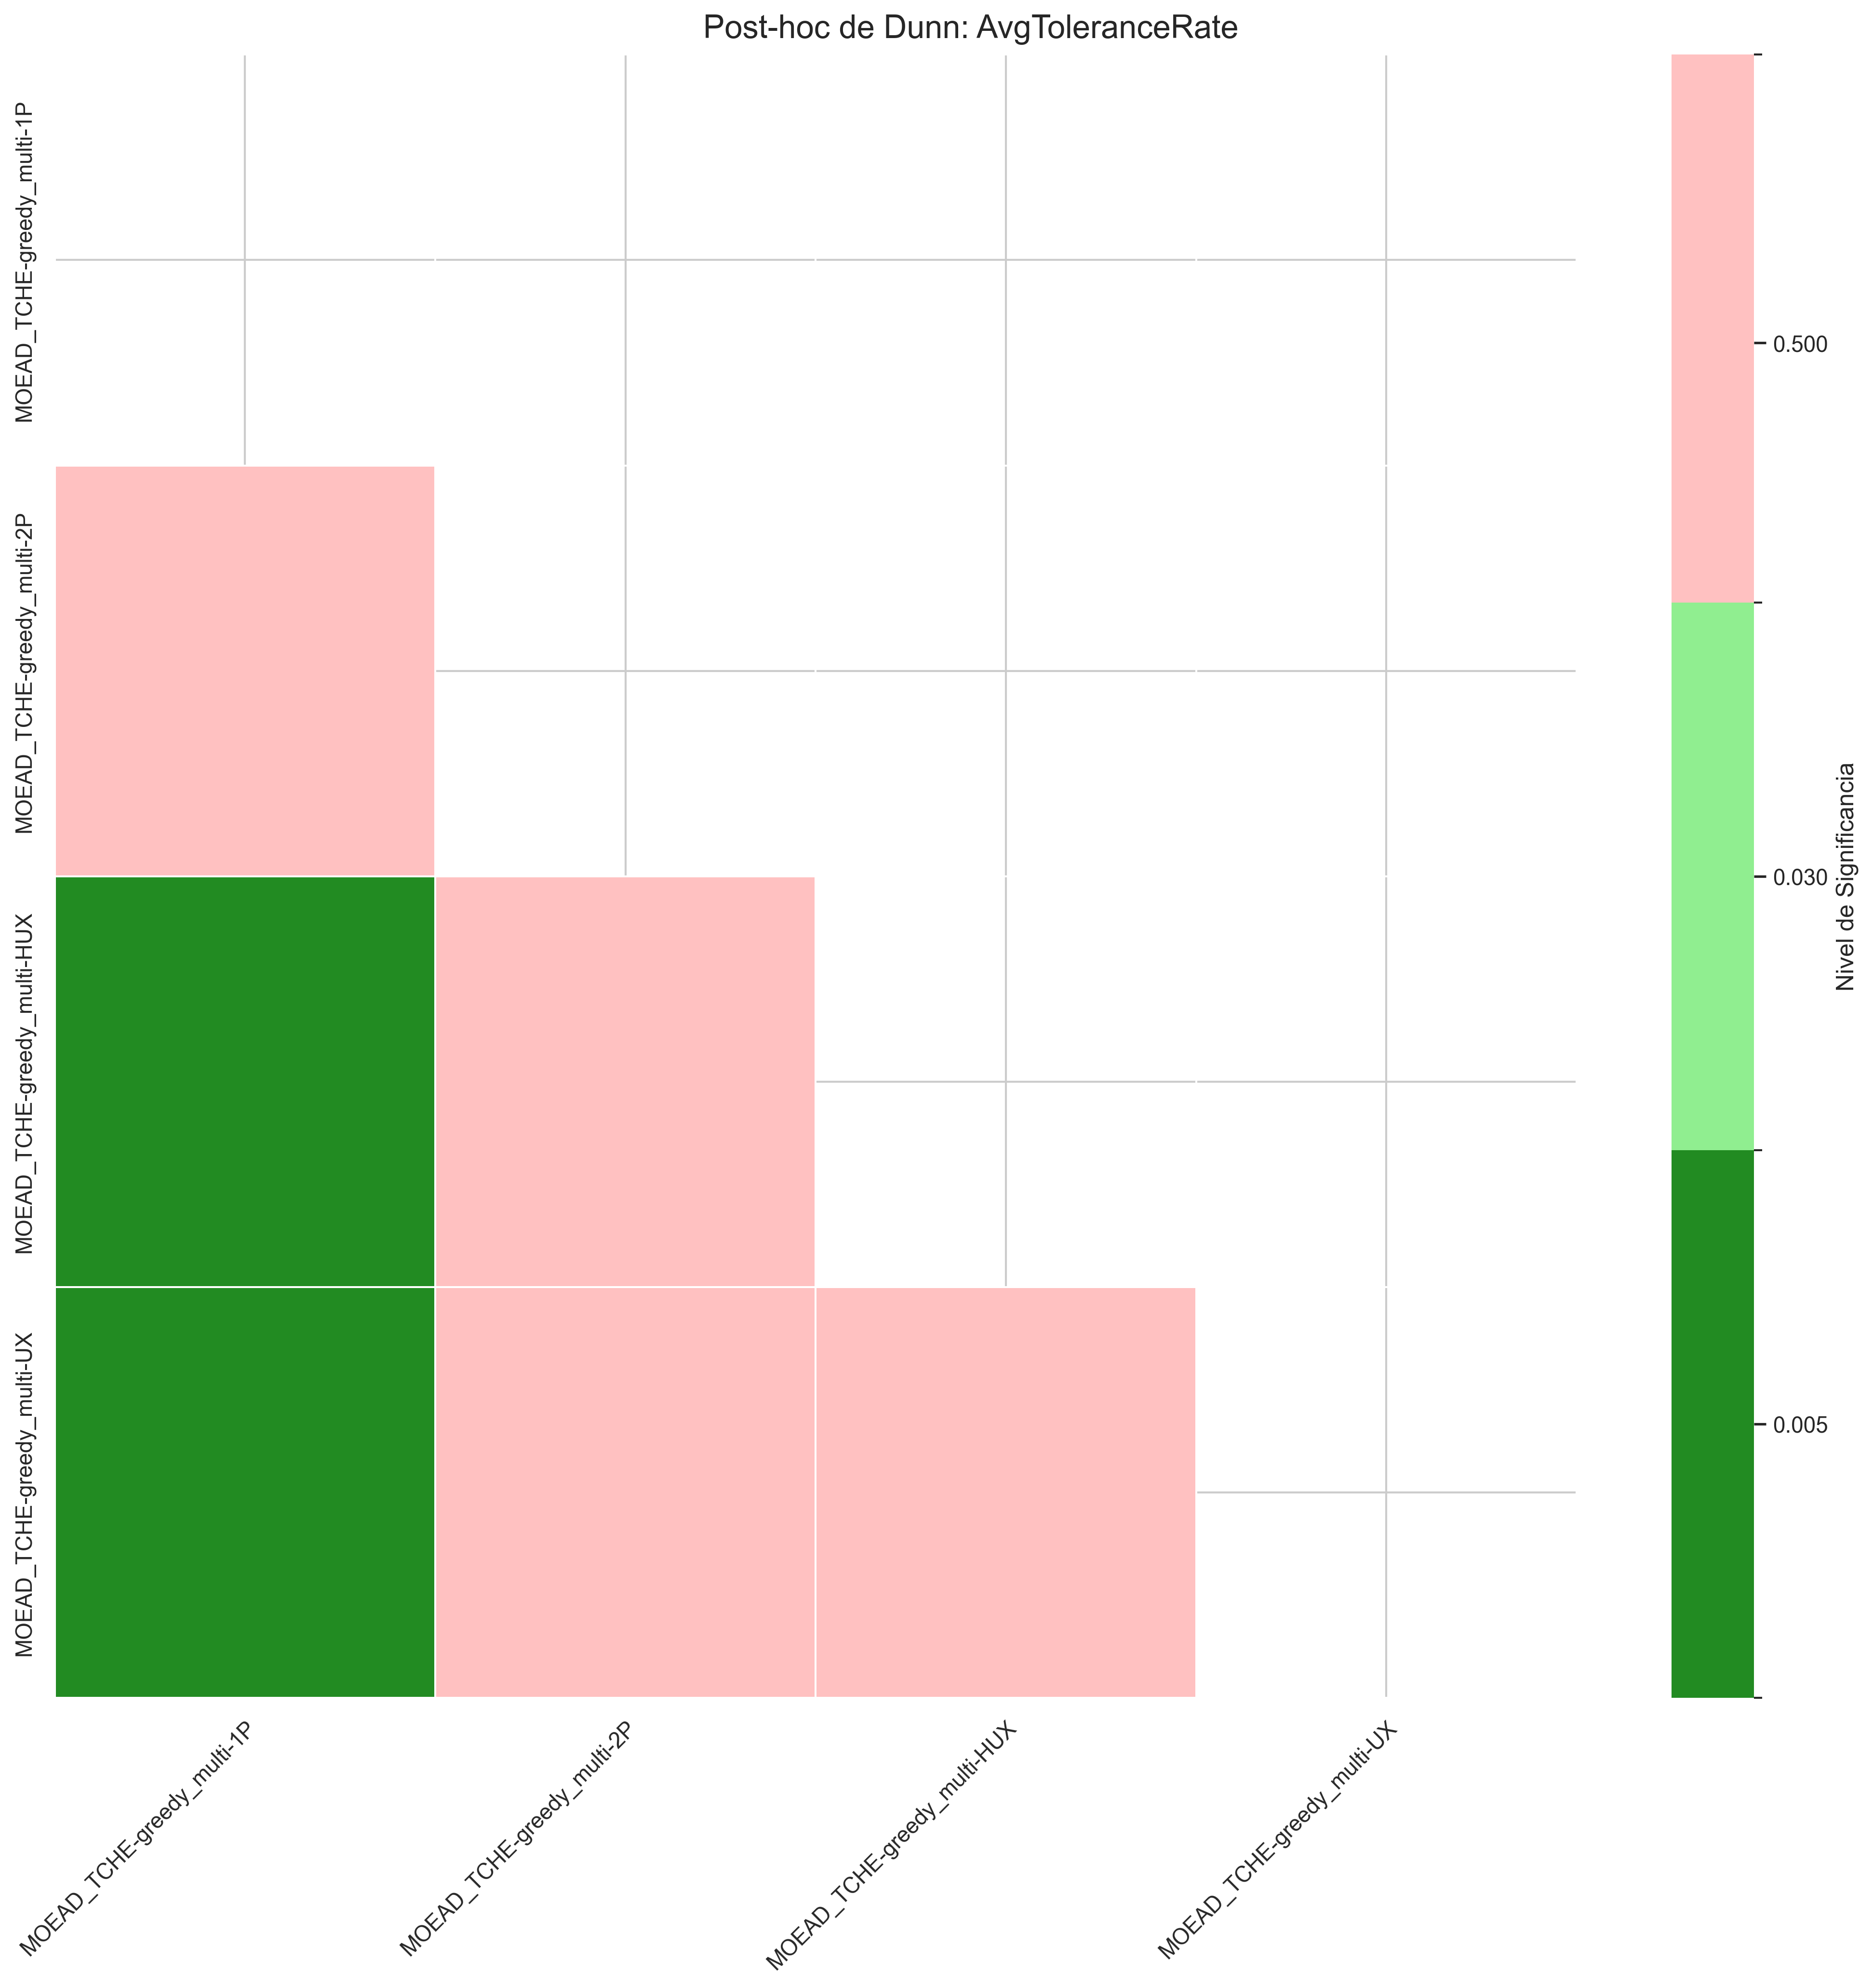
\includegraphics[width=\textwidth]{../exp_auxiliares/full20_cx_negAbs/2_comparativa/4_rankings/estadistica_hv/heatmap_dunn_avgtolerancerate_full_20.png}
        \caption{Test de Dunn con 20 runs}
        \label{fig:dunn_atr_20runs}
    \end{subfigure}
    \hfill
    \begin{subfigure}[b]{0.48\textwidth}
        \centering
        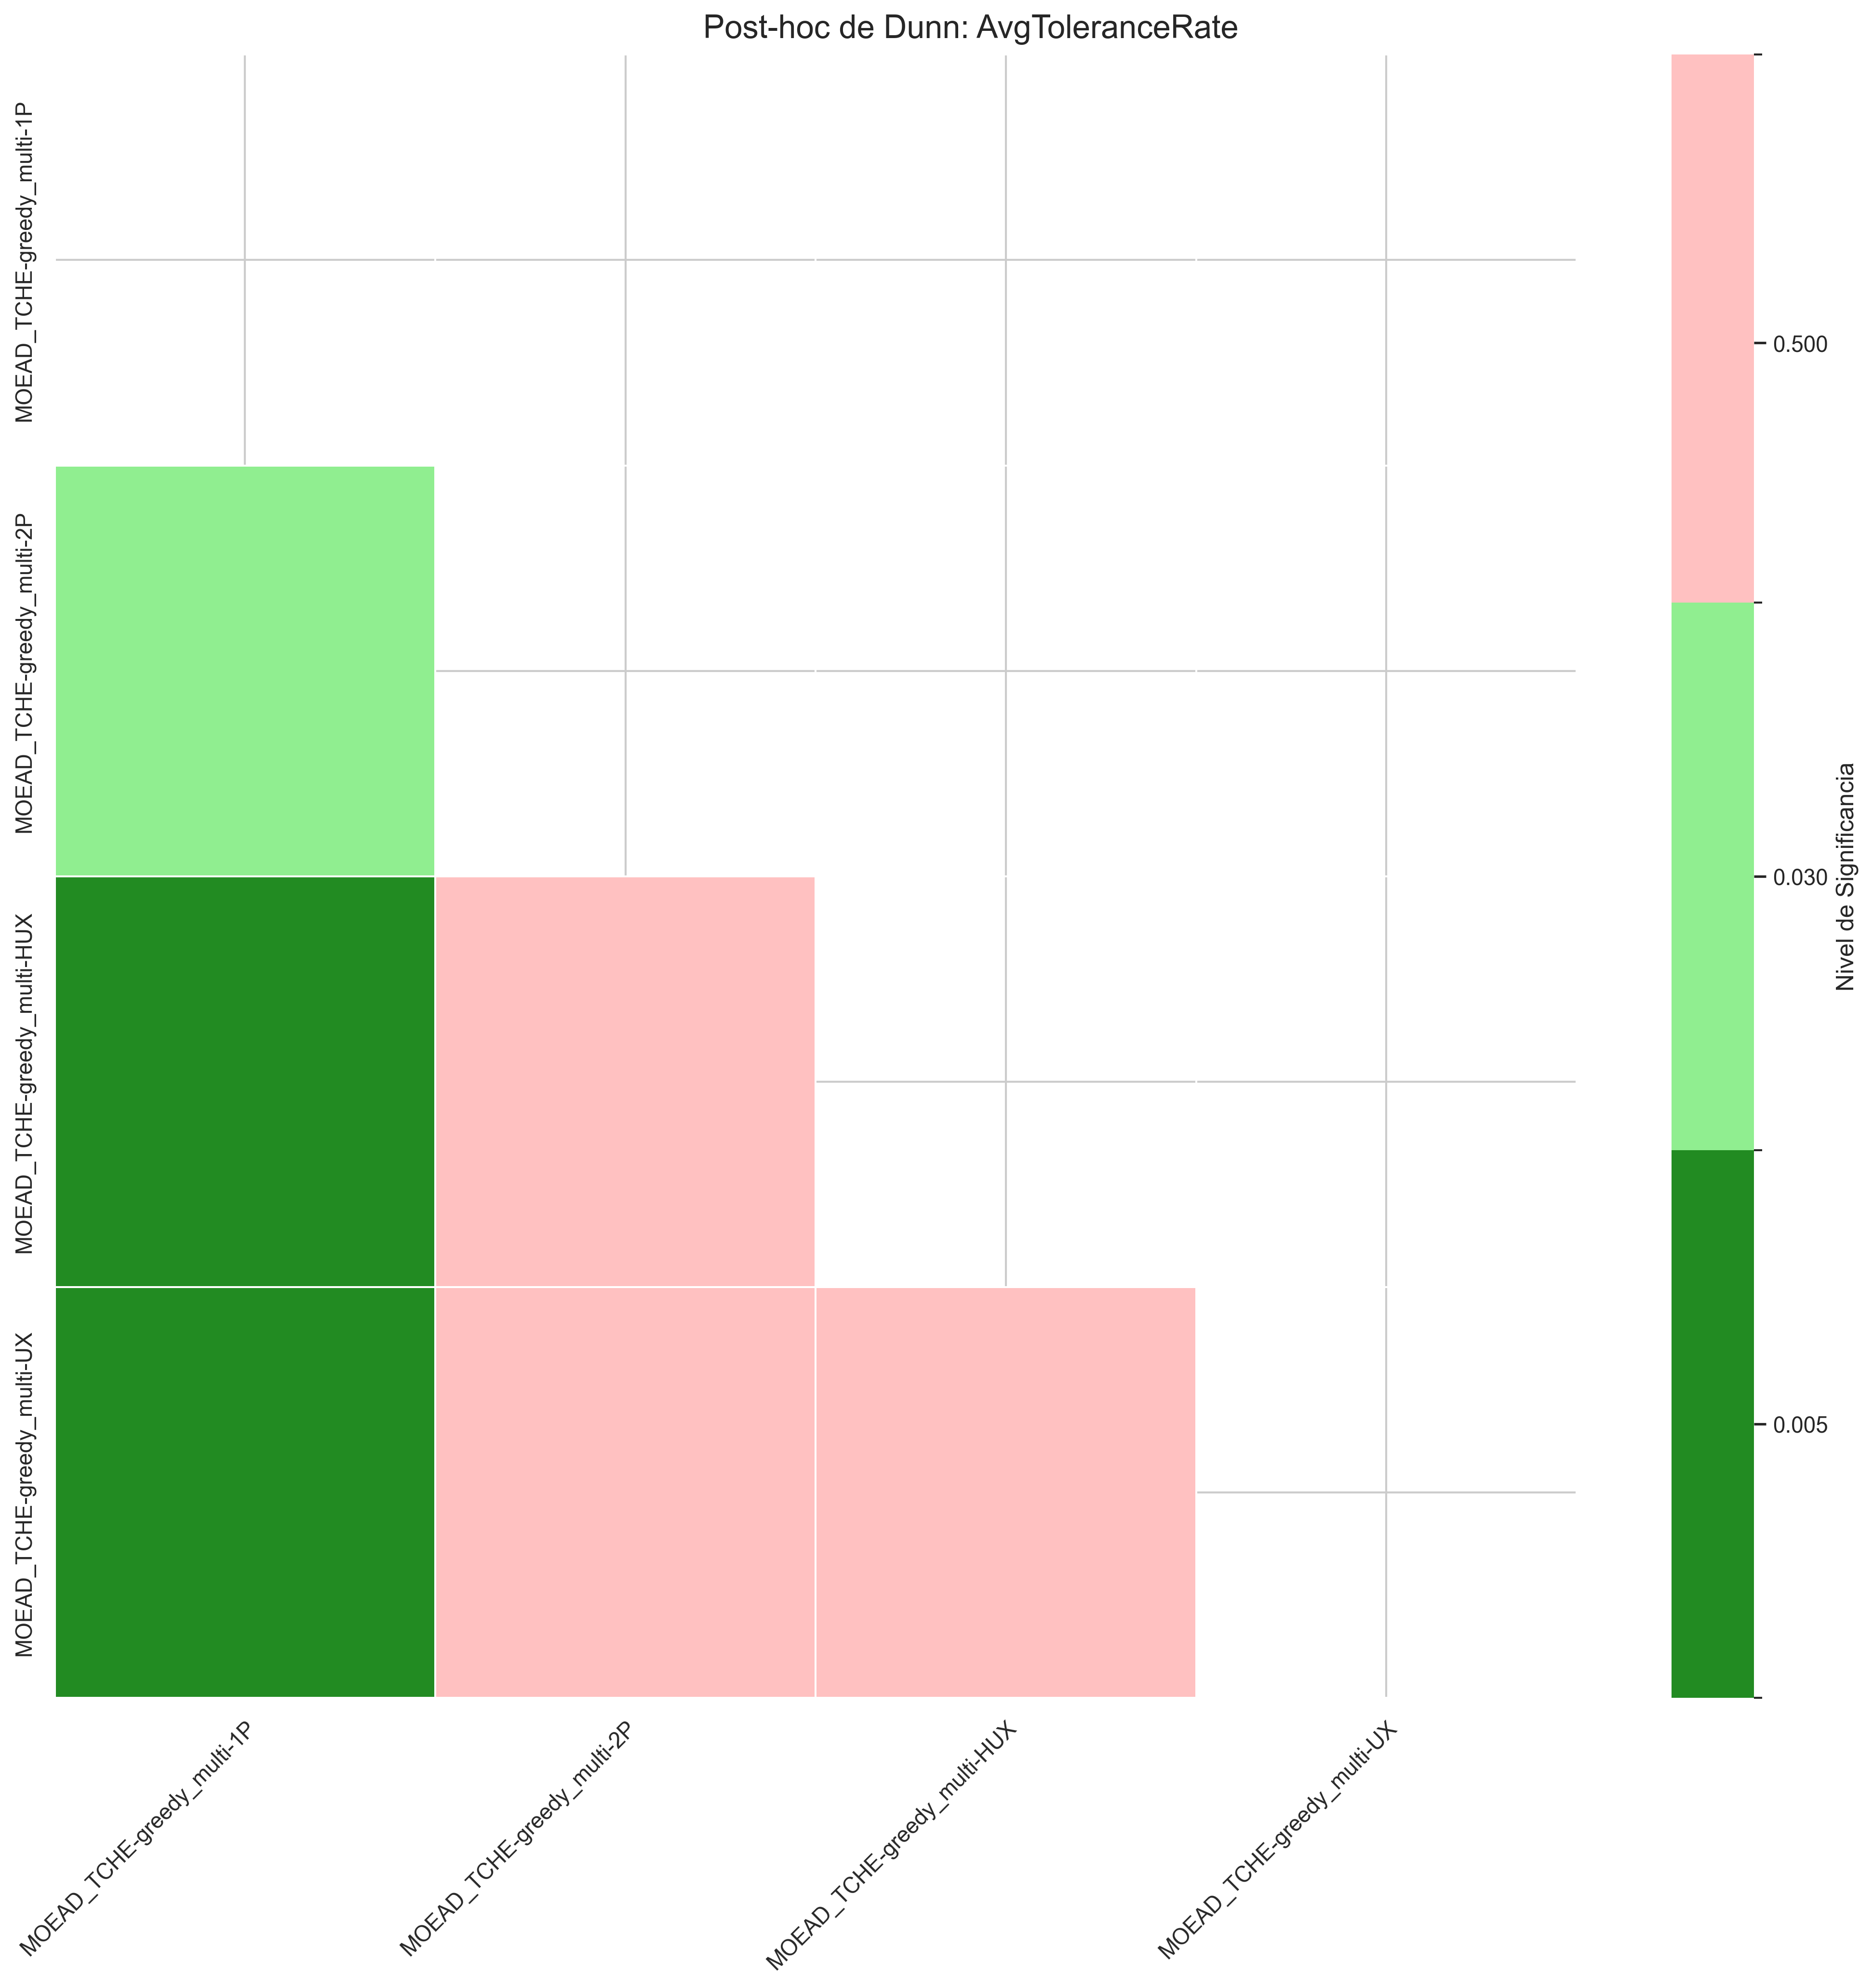
\includegraphics[width=\textwidth]{../exp_auxiliares/full30_cx_negAbs/2_comparativa/4_rankings/estadistica_hv/heatmap_dunn_avgtolerancerate_full_30.png}
        \caption{Test de Dunn con 30 runs}
        \label{fig:dunn_atr_30runs}
    \end{subfigure}
    \caption{Comparativa del análisis post hoc (Test de Dunn) para la métrica Avg Tolerance Rate con 20 y 30 runs. Con 20 runs se distinguen 2 de 6 pares, mientras que con 30 runs se añade un nuevo par significativo, alcanzando 3 de 6 pares.}
    \label{fig:dunn_20vs30_atr}
\end{figure}

\subsubsection{Trade-off coste computacional}

El incremento de 20 a 30 runs supone un aumento del tiempo de ejecución de aproximadamente un 38\% (de $\sim$1h 10min a $\sim$1h 36min). Cabe señalar que la métrica IGD+ permanece no significativa en ambos escenarios ($p = 0.816$ con 20 runs y $p = 0.886$ con 30 runs), lo que sugiere que ciertas métricas requieren un tamaño muestral aún mayor o presentan una varianza inherente que no se reduce con más semillas.

\subsubsection{Conclusión y decisión pendiente}

La evidencia empírica sugiere que 30 runs constituye un mínimo razonable para garantizar una discriminación post hoc robusta entre la mayoría de las configuraciones. No se dispone de evidencia empírica con más de 30 runs que permita evaluar si un incremento adicional (por ejemplo, 50 o 100 runs) aportaría beneficios sustanciales. La decisión final sobre el número de runs para el experimento definitivo se deja a tu criterio, considerando las restricciones temporales y computacionales del proyecto.


\clearpage
\section{Decisiones pendientes y aprobación}

A lo largo de este documento técnico se han expuesto y analizado rigurosamente diversas configuraciones y parámetros para la ejecución del experimento general definitivo. A modo de síntesis, las principales decisiones que quedan supeditadas a tu revisión y aprobación son las siguientes:

\begin{itemize}
    \item \textbf{Espacio algorítmico:} Se propone un abanico de 7 algoritmos multiobjetivo (NSGA-II, NSGA-III, SPEA2, MOEA/D-TCHE, AGE-MOEA2, SMS-EMOA, RVEA), 2 estrategias de inicialización y 4 operadores de cruce (56 combinaciones en total). Queda a tu discreción añadir, sustituir o suprimir cualquier algoritmo o configuración de esta lista.
    \item \textbf{Ajuste del hipervolumen:} La adopción de un punto de referencia $R = [1.1, 1.1, 1.1, 1.1]$ se considera fundamental para no invisibilizar a las soluciones extremas y evitar una evaluación sesgada del rendimiento.
    \item \textbf{Modo de evaluación y transformaciones:} La evidencia y el sustento teórico apuntan fuertemente al uso del \textbf{modo absoluto} acoplado con una \textbf{transformación matemática de negación} ($-x$), frente al modo proporcional y a la inversión ($1/x$), para preservar eficazmente la diversidad del espacio fenotípico.
    \item \textbf{Tamaño muestral:} Se presenta evidencia empírica comparando ejecuciones de 20 y 30 \textit{runs} independientes. Aunque 30 semillas ofrecen una potencia estadística notablemente superior en el análisis \textit{post hoc} para establecer una jerarquía algorítmica clara, se deja la decisión final en función de los recursos computacionales y temporales del proyecto.
\end{itemize}

Quedo a tu entera disposición para discutir e integrar cualquier aportación técnica, adición algorítmica u observación adicional que consideres oportuna antes del inicio oficial del experimento general.

\end{document}
